% === ICMLarXiv.tex ===
%%%%%%%% ICML 2026 EXAMPLE LATEX SUBMISSION FILE %%%%%%%%%%%%%%%%%

\documentclass{article}

% Recommended, but optional, packages for figures and better typesetting:
\usepackage{microtype}
\usepackage{graphicx}
\usepackage{subcaption}
\usepackage{booktabs} % for professional tables
\usepackage{pifont}
\usepackage{float}

% hyperref makes hyperlinks in the resulting PDF.
% If your build breaks (sometimes temporarily if a hyperlink spans a page)
% please comment out the following usepackage line and replace
% \usepackage{icml2026} with \usepackage[nohyperref]{icml2026} above.
\usepackage{hyperref}


% Attempt to make hyperref and algorithmic work together better:
\newcommand{\theHalgorithm}{\arabic{algorithm}}

% Use the following line for the initial blind version submitted for review:
\usepackage[accepted]{icml2026}

% For preprint, use
% \usepackage[preprint]{icml2026}

% If accepted, instead use the following line for the camera-ready submission:
% \usepackage[accepted]{icml2026}

\usepackage{amsmath}
\usepackage{amssymb}
\usepackage{mathtools}
\usepackage{amsthm}
\usepackage{algorithm,algorithmic}
\usepackage{listings}
\lstset{
	language=Python,
	basicstyle=\ttfamily\small,
	keywordstyle=\color{blue!70!black},
	stringstyle=\color{orange!70!black},
	commentstyle=\itshape\color{green!50!black},
	showstringspaces=false,
	breaklines=true,
	numbers=left,
	numberstyle=\tiny\color{gray},
	frame=single,
	tabsize=4
}

\newcommand{\RETURN}{\STATE \textbf{return}}

\usepackage{tikz}
\usetikzlibrary{shapes.geometric, arrows.meta, positioning, fit, calc, backgrounds, shadows}

% 定义风格配色
\definecolor{s5blue}{RGB}{70, 130, 180}   % Learnable parameters
\definecolor{s5green}{RGB}{85, 107, 47}   % Instantiated variables
\definecolor{s5purple}{RGB}{128, 0, 128}  % Data flow
\definecolor{s5box}{RGB}{250, 250, 250}   % Background fill


% if you use cleveref..
\usepackage[capitalize,noabbrev]{cleveref}

%%%%%%%%%%%%%%%%%%%%%%%%%%%%%%%%
% THEOREMS
%%%%%%%%%%%%%%%%%%%%%%%%%%%%%%%%
\theoremstyle{plain}
\newtheorem{theorem}{Theorem}[section]
\newtheorem{proposition}[theorem]{Proposition}
\newtheorem{lemma}[theorem]{Lemma}
\newtheorem{corollary}[theorem]{Corollary}
\theoremstyle{definition}
\newtheorem{definition}[theorem]{Definition}
\newtheorem{assumption}[theorem]{Assumption}
\theoremstyle{remark}
\newtheorem{remark}[theorem]{Remark}
\DeclareMathOperator*{\argmin}{arg\,min}

% Todonotes is useful during development; simply uncomment the next line
%    and comment out the line below the next line to turn off comments
%\usepackage[disable,textsize=tiny]{todonotes}
\usepackage[textsize=tiny]{todonotes}

% The \icmltitle you define below is probably too long as a header.
% Therefore, a short form for the running title is supplied here:
\icmltitlerunning{FRACTAL: SSM with Fractional Recurrent Architecture for Computational Temporal Analysis of Long Sequences}

\begin{document}

\twocolumn[
  \icmltitle{FRACTAL: State Space Model with Fractional Recurrent Architecture \\
  	for Computational Temporal Analysis of Long Sequences}

  % It is OKAY to include author information, even for blind submissions: the
  % style file will automatically remove it for you unless you've provided
  % the [accepted] option to the icml2026 package.

  % List of affiliations: The first argument should be a (short) identifier you
  % will use later to specify author affiliations Academic affiliations
  % should list Department, University, City, Region, Country Industry
  % affiliations should list Company, City, Region, Country

  % You can specify symbols, otherwise they are numbered in order. Ideally, you
  % should not use this facility. Affiliations will be numbered in order of
  % appearance and this is the preferred way.
  \icmlsetsymbol{equal}{*}

  \begin{icmlauthorlist}
  	\icmlauthor{Mengqi Li}{nwpu}
  	\icmlauthor{Wensheng Lin}{nwpu,dk}
  	\icmlauthor{Jinshuai Yang}{nwpu}
  	\icmlauthor{Lixin Li}{nwpu,dk}
%    \icmlauthor{Firstname1 Lastname1}{equal,yyy}
%    \icmlauthor{Firstname2 Lastname2}{equal,yyy,comp}
%    \icmlauthor{Firstname3 Lastname3}{comp}
%    \icmlauthor{Firstname4 Lastname4}{sch}
%    \icmlauthor{Firstname5 Lastname5}{yyy}
%    \icmlauthor{Firstname6 Lastname6}{sch,yyy,comp}
%    \icmlauthor{Firstname7 Lastname7}{comp}
%    %\icmlauthor{}{sch}
%    \icmlauthor{Firstname8 Lastname8}{sch}
%    \icmlauthor{Firstname8 Lastname8}{yyy,comp}
    %\icmlauthor{}{sch}
    %\icmlauthor{}{sch}
  \end{icmlauthorlist}

  %\icmlaffiliation{*}{Equal contribution}
  \icmlaffiliation{nwpu}{School of Electronics and Information,
  	Northwestern Polytechnical University, Xi'an, Shaanxi, China.}
  \icmlaffiliation{dk}{DecoreX Intelligent Technologies Co., Ltd., Xi'an 710075 China}
  
  \icmlcorrespondingauthor{Lixin Li}{lilixin@nwpu.edu.cn}
  \icmlcorrespondingauthor{Wensheng Lin}{linwest@nwpu.edu.cn}

  % You may provide any keywords that you find helpful for describing your
  % paper; these are used to populate the "keywords" metadata in the PDF but
  % will not be shown in the document
  \icmlkeywords{Machine Learning, ICML}

  \vskip 0.3in
]

% this must go after the closing bracket ] following \twocolumn[ ...

% This command actually creates the footnote in the first column listing the
% affiliations and the copyright notice. The command takes one argument, which
% is text to display at the start of the footnote. The \icmlEqualContribution
% command is standard text for equal contribution. Remove it (just {}) if you
% do not need this facility.

% Use ONE of the following lines. DO NOT remove the command.
% If you have no special notice, KEEP empty braces:
\printAffiliationsAndNotice{}  % no special notice (required even if empty)
% Or, if applicable, use the standard equal contribution text:
% \printAffiliationsAndNotice{\icmlEqualContribution}

\begin{abstract}
	Effective sequence modeling fundamentally requires balancing the retention of unbounded history with the high-resolution detection of abrupt short-term variations common in real-world phenomena. However, existing state space models (SSMs) relying on high-order polynomial projection operators (HiPPO) face a critical trade-off where uniform measures dilute recent information to maintain timescale invariance, while exponential measures sacrifice global context to capture local dynamics. This paper proposes a Fractional Recurrent Architecture for Computational Temporal Analysis of Long sequences (FRACTAL), a novel architecture integrating fractional measure theory into recursive memory updates to address this limitation. By deriving projection operators with analytically characterized spectral properties and a tunable singularity index, the proposed method amplifies sensitivity to recent signal perturbations while preserving the spectral structure that encodes scale-invariant memory dynamics. This theoretical innovation is instantiated within a simplified diagonalized state space framework by modulating input projection initialization to enable simultaneous capture of multi-scale temporal features.  FRACTAL achieves an average score of 87.11\% on the Long Range Arena benchmark, including 61.85\% on the ListOps task, outperforming the S5 model.
	%FRACTAL improves the challenging ListOps task to 61.85\%, which outperforms S5.
\end{abstract}

\section{Introduction}
\label{sec:intro}
Sequence modeling in continuous time requires resolving the fundamental tension between retention of unbounded historical context and high-resolution detection of recent input perturbations. While Long Short-Term Memory networks~\citep{hochreiter1997long} and Transformers~\citep{vaswani2017attention} address these aspects through distinct mechanisms, state space models (SSMs) have emerged as a unified framework offering linear scaling complexity and rigorous grounding in continuous signal processing~\citep{gu2022efficiently, tay2021long}. The theoretical foundation of modern SSMs lies in the high-order polynomial projection operators (HiPPO) framework~\citep{gu2020hippo}, which formalizes memory as an online polynomial approximation problem governed by a probability measure. This measure serves as the primary mechanism determining the memory profile by dictating how the system weights historical information relative to the present.

Despite rapid architectural evolution from structured matrices~\citep{gu2022efficiently, gupta2022diagonal} to selective state spaces~\citep{gu2024mamba}, the foundational choice of measure remains largely unexplored. Existing HiPPO instantiations present a critical trilemma. The \textit{Scaled Legendre} measure (LegS) assigns uniform weight to history, ensuring timescale invariance but progressively diluting the influence of recent inputs as time advances. The \textit{Translated Laguerre} measure (LagT) prioritizes recency via exponential decay but imposes a fixed characteristic timescale that sacrifices robustness to time-warped signals. The \textit{Translated Legendre} measure (LegT)~\citep{voelker2019legendre} provides high local resolution but catastrophically discards context beyond a fixed sliding window.

This theoretical gap limits the applicability of SSMs in physical and biological domains characterized by multi-scale dynamics. Real-world phenomena ranging from volatility clustering in financial markets~\citep{mandelbrot1997multifractal} and $1/f$ noise in physiological signals~\citep{west2010fractal}, to the bursty nature of network traffic~\citep{leland1994self}, exhibit long memory characteristics defined by power-law decay kernels. Such systems possess a heavy tail of history that interacts non-linearly with abrupt local variations. Standard SSMs governed by integer-order differential equations inherently impose exponential memory decay via LagT or uniform averaging via LegS, creating an impedance mismatch with these scale-free natural processes.

\begin{figure*}[t]
	\centering
	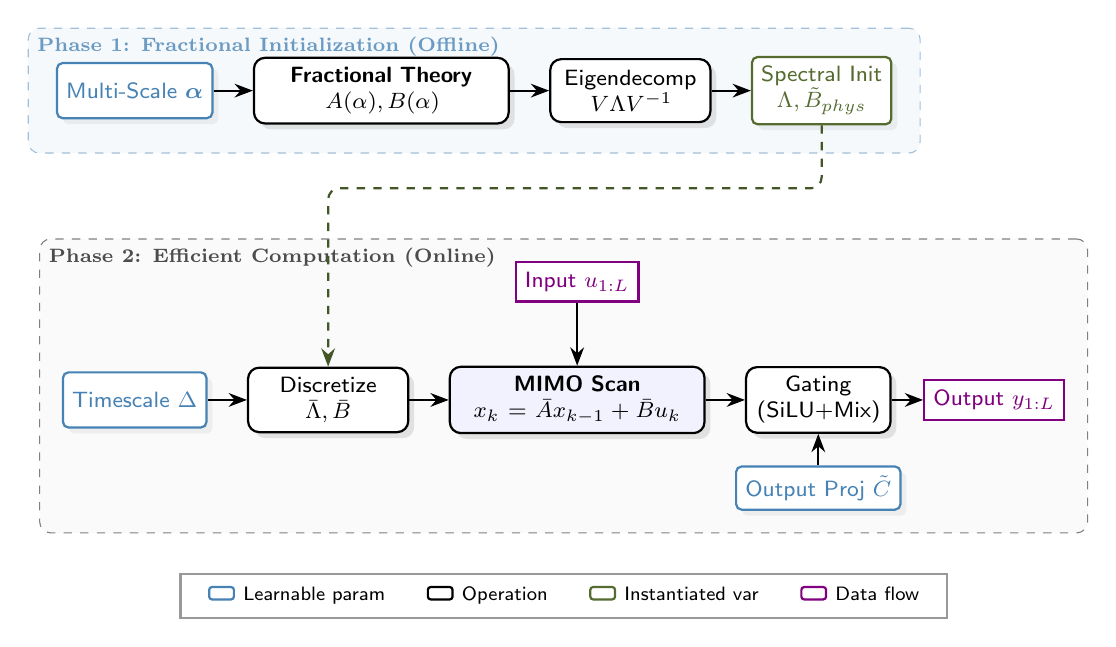
\begin{tikzpicture}[
		% 全局设置
		node distance=0.8cm and 0.5cm, % 稍微缩短水平间距使箭头更短
		font=\footnotesize\sffamily,
		% 样式定义
		param/.style={rectangle, draw=s5blue, text=s5blue, thick, rounded corners=2pt, minimum width=1.6cm, minimum height=0.7cm, align=center, fill=white, drop shadow={opacity=0.1}},
		var/.style={rectangle, draw=s5green, text=s5green, thick, rounded corners=2pt, minimum width=1.6cm, minimum height=0.7cm, align=center, fill=white, drop shadow={opacity=0.1}},
		op/.style={rectangle, draw=black, thick, rounded corners=4pt, minimum width=1.8cm, minimum height=0.8cm, align=center, fill=white, drop shadow={opacity=0.2}, text width=1.8cm},
		data/.style={rectangle, draw=s5purple, text=s5purple, thick, minimum width=1.2cm, minimum height=0.5cm, fill=white, align=center},
		arrow/.style={-Stealth, thick, rounded corners},
		line/.style={thick}
		]
		
		% ==========================================
		% Phase 1: Initialization (Top Row)
		% ==========================================
		
		% 1. 输入 Alpha
		\node[param] (alpha) {Multi-Scale $\boldsymbol{\alpha}$};
		
		% 2. 理论计算
		\node[op, right=of alpha, text width=3cm] (theory) {\textbf{Fractional Theory}\\$A(\alpha), B(\alpha)$};
		
		% 3. 特征分解
		\node[op, right=of theory] (eig) {Eigendecomp\\$V \Lambda V^{-1}$};
		
		% 4. 物理初始化结果
		\node[var, right=of eig] (init_vars) {Spectral Init\\$\Lambda, \tilde{B}_{phys}$};
		
		% 连接线 Phase 1
		\draw[arrow] (alpha) -- (theory);
		\draw[arrow] (theory) -- (eig);
		\draw[arrow] (eig) -- (init_vars);
		
		% ==========================================
		% Phase 2: Online Computation (Bottom Row)
		% ==========================================
		
		% 关键修改：垂直距离增加到 3.2cm，确保 Input 不会撞到上面的框
		\node[param, below=3.2cm of alpha] (delta) {Timescale $\Delta$};
		
		% 6. 离散化
		\node[op, right=of delta] (zoh) {Discretize\\$\bar{\Lambda}, \bar{B}$};
		
		% 7. 并行扫描 (核心模块)
		\node[op, right=of zoh, minimum width=2.2cm, fill=blue!5, text width=3cm] (scan) {\textbf{MIMO Scan}\\$x_k = \bar{A}x_{k-1} + \bar{B}u_k$};
		
		% 8. 输入数据 Input (现在有足够的空间了)
		\node[data, above=0.8cm of scan] (input) {Input $u_{1:L}$};
		
		% 9. 混合与输出
		\node[op, right=of scan, text width=1.6cm] (glu) {Gating\\(SiLU+Mix)};
		\node[data, right=0.4cm of glu] (output) {Output $y_{1:L}$};
		
		% 学习参数 C
		\node[param, below=0.4cm of glu, minimum height=0.5cm] (C) {Output Proj $\tilde{C}$};
		
		% 连接线 Phase 2
		\draw[arrow] (delta) -- (zoh);
		\draw[arrow] (zoh) -- (scan);
		\draw[arrow] (input) -- (scan);
		\draw[arrow] (scan) -- (glu);
		\draw[arrow] (glu) -- (output);
		\draw[arrow] (C) -- (glu);
		
		% ==========================================
		% 跨层连接 (Phase 1 -> Phase 2)
		% ==========================================
		% 路径优化：直角连接，避开 Input 节点
		\draw[arrow, s5green!80!black, dashed] (init_vars.south) -- ++(0,-0.8) -| (zoh.north);
		
		% ==========================================
		% 背景框 (Background Boxes)
		% ==========================================
		\begin{scope}[on background layer]
			% Phase 1 Box
			\node[fit=(alpha)(theory)(eig)(init_vars), 
			draw=s5blue!50, dashed, fill=s5blue!5, rounded corners, inner sep=10pt,
			label={[anchor=north west, text=s5blue!80, font=\scriptsize\bfseries]north west:Phase 1: Fractional Initialization (Offline)}] (box_init) {};
			
			% Phase 2 Box (包含 input 节点)
			\node[fit=(delta)(zoh)(scan)(glu)(output)(C)(input), 
			draw=black!50, dashed, fill=black!2, rounded corners, inner sep=8pt,
			label={[anchor=north west, text=black!70, font=\scriptsize\bfseries]north west:Phase 2: Efficient Computation (Online)}] (box_run) {};
		\end{scope}
		
		% ==========================================
		% Legend (图例) - 移至最下方，独立于 Phase 2
		% ==========================================
		% 参考 S5 Figure 1 的底部图例风格
		
		\node[draw=black!40, thick, fill=white, rounded corners=0pt, anchor=north, yshift=-0.5cm, inner sep=4pt] at (box_run.south) {
			\scriptsize
			\begin{tabular}{c@{\hskip 3pt}l @{\hskip 15pt} c@{\hskip 3pt}l @{\hskip 15pt} c@{\hskip 3pt}l @{\hskip 15pt} c@{\hskip 3pt}l}
				% Learnable Parameter (Blue Rect)
				\tikz\node[draw=s5blue, thick, fill=white, minimum width=1.2em, minimum height=0.6em, inner sep=0pt, rounded corners=1pt]{}; & Learnable param &
				
				% Operation (Black Rect - 统一为矩形，看起来更整齐)
				\tikz\node[draw=black, thick, fill=white, minimum width=1.2em, minimum height=0.6em, inner sep=0pt, rounded corners=1pt]{}; & Operation &
				
				% Instantiated Variable (Green Rect)
				\tikz\node[draw=s5green, thick, fill=white, minimum width=1.2em, minimum height=0.6em, inner sep=0pt, rounded corners=1pt]{}; & Instantiated var &
				
				% Data Flow (Purple Rect)
				\tikz\node[draw=s5purple, thick, fill=white, minimum width=1.2em, minimum height=0.6em, inner sep=0pt, rounded corners=1pt]{}; & Data flow
			\end{tabular}
		};
		
	\end{tikzpicture}
	\caption{The computational architecture of FRACTAL. \textbf{Top (Phase 1):} Offline initialization. The multi-scale $\boldsymbol{\alpha}$ derives fractional operators, spectrally decomposed to produce $\Lambda$ and a physically-informed $\tilde{B}_{phys}$. \textbf{Bottom (Phase 2):} Online computation. The instantiated parameters are discretized and executed via efficient MIMO parallel scans.}
	\label{fig:fractal_arch}
\end{figure*}

Bridging this gap motivates the adoption of fractional calculus, a mathematical framework generalizing differentiation to non-integer orders. Unlike integer-order operators that imply local dependencies, fractional operators naturally describe non-local memory and hereditary properties~\citep{podlubny1998fractional}. A fractional-order measure provides a rigorous interpolation mechanism wherein adjusting the singularity index continuously tunes the memory kernel between a uniform distribution (pure history) and concentrated mass at the present (pure recency). This observation motivates FRACTAL (Fractional Recurrent Architecture for Computational Temporal Analysis of Long sequences), illustrated in Figure~\ref{fig:fractal_arch}. The proposed approach generalizes the measure-theoretic foundation of SSMs by introducing a fractional-order measure with a tunable singularity index $\alpha \in [0, 1)$. In contrast to exponential decay, this measure induces a power-law weighting $(t-\tau)^{-\alpha}$ that creates a heavy tail for long-term retention while mathematically enforcing a singularity at the current timestep to amplify local sensitivity.

\paragraph{Related Work.}
\label{sec:related_work}

The evolution of efficient sequence modeling has largely focused on computational tractability rather than measure-theoretic fundamentals. The Legendre Memory Unit (LMU)~\citep{voelker2019legendre} pioneered the use of orthogonal projections derived from delay differential equations but was restricted to fixed sliding windows. The S4 model~\citep{gu2022efficiently} extended this to infinite history using HiPPO-LegS matrices decomposed into Normal Plus Low-Rank (NPLR) structures, enabling efficient convolution via FFT. Subsequent simplifications, such as S4D~\citep{gu2022parameterization}, DSS~\citep{gupta2022diagonal}, and S5~\citep{smith2023simplified}, demonstrated that the precise matrix structure is secondary to spectral properties, advocating for diagonalized Multi-Input Multi-Output (MIMO) systems initialized with HiPPO spectra. However, these works treat the HiPPO matrix as a static initialization artifact, ignoring the potential of the underlying measure to serve as a dynamic design parameter.

Parallel to the SSM development, fractional calculus has explored memory modeling, albeit often heuristically. 
Fractional gradient methods~\citep{wang2017fractional} introduced fractional-order derivatives into backpropagation to impose heavy-tailed memory on weight updates, though this approach focuses on optimization rather than sequence representation. 
In the domain of continuous dynamics, Physics-Informed Neural Networks have been rigorously extended to fractional orders (fPINNs)~\citep{pang2019fpinns} to solve fractional differential equations. 
However, these approaches typically rely on expensive numerical solvers or automatic differentiation through fractional operators, rendering them computationally prohibitive for large-scale sequence modeling tasks. 
% The present work bridges these lineages by leveraging the optimal projection theory of HiPPO together with the memory properties of fractional calculus to derive an efficient state space parameterization with an analytically characterized spectral structure.
The present work bridges these lineages by leveraging the optimal projection theory of HiPPO together with the memory properties of fractional calculus to derive an efficient state-space parameterization with an analytically characterized spectral structure.

The SSM landscape has recently bifurcated into two orthogonal paradigms. \textit{Selective} (time-varying) SSMs, such as Mamba~\citep{gu2024mamba} and DeltaNet, achieve strong empirical performance by making the state-transition matrices input-dependent, effectively enabling data-dependent gating. These architectures are predominantly designed as generative language model backbones relying on large-scale pre-training and hardware-aware scan implementations. \textit{Linear Time-Invariant} (LTI) SSMs (S4, S4D, DSS, S5, and this work) instead focus on the continuous-time mathematical measure $\mu^{(t)}$ used to compress history, and are evaluated by training from scratch to isolate the pure structural inductive bias of the sequence mixer. FRACTAL belongs strictly to the LTI category. Comparing a foundational, train-from-scratch LTI innovation against heavily optimised, pre-trained selective architectures conflates two distinct research paradigms and would obscure the specific theoretical contribution of the fractional measure; S5 therefore remains the appropriate rigorous baseline.

\paragraph{Our Contributions.}
\label{sec:contributions}

This paper makes three contributions:

%(1) \textbf{Theory.} A fractional-order measure is introduced that generalizes the HiPPO framework. This measure assigns power-law weights to historical timesteps, with a single parameter controlling the trade-off between uniform coverage and recency emphasis. The corresponding orthogonal basis consists of Jacobi polynomials with explicit normalization constants. The resulting state transition matrix $A(\alpha)$ exhibits a key structural property in which the diagonal elements equal $n+1$ independent of $\alpha$, guaranteeing spectral stability. The input projection vector $B(\alpha)$ admits a complete closed-form solution in terms of generalized binomial coefficients.
%
%(2) \textbf{Architecture.} The FRACTAL architecture operationalizes this theoretical framework within a multi-input multi-output structure amenable to parallel computation. A multi-channel configuration assigns heterogeneous memory parameters across state dimensions, enabling the simultaneous capture of patterns at multiple temporal scales.
%
%(3) \textbf{Experiments.} Comprehensive experiments on the Long Range Arena benchmark and additional sequence modeling tasks validate the proposed approach.
%Results demonstrate state-of-the-art performance on tasks requiring long-range reasoning, confirming the importance of fractional-order memory and multi-scale parameterization.


(1) \textbf{Theory.} We introduce a fractional-order power-law measure into the HiPPO projection framework as the first measure to simultaneously satisfy full-history retention, recency sensitivity, and scale invariance, by placing an integrable singularity at the current time while maintaining the polynomial decay over distant history that scale invariance structurally requires. Rigorous derivation of the resulting state-space dynamics establishes that Jacobi polynomials form the natural orthonormal basis, that the eigenvalues of the state transition matrix are invariant to the singularity index for all admissible parameter values, and that the input projection admits a complete closed-form solution.

(2) \textbf{Architecture.} The FRACTAL architecture operationalizes this theoretical framework within a multi-input multi-output structure amenable to parallel computation. A multi-channel configuration assigns heterogeneous memory parameters across state dimensions, enabling the simultaneous capture of patterns at multiple temporal scales.

(3) \textbf{Experiments.} Comprehensive experiments on the Long Range Arena benchmark validate the proposed approach. Results demonstrate state-of-the-art performance on tasks requiring long-range reasoning, validating the impact of fractional-order memory and multi-scale parameterization.
\section{Background}
\label{sec:background}

This section reviews the theoretical foundations of state space models and the HiPPO framework, emphasizing the role of measures in shaping memory dynamics.

\subsection{Linear State Space Models}
\label{subsec:ssm}

Continuous-time linear SSMs map an input $u(t) \in \mathbb{R}$ to an output $y(t) \in \mathbb{R}$ via a latent state $x(t) \in \mathbb{R}^N$ using the equations:
\begin{equation}
	\frac{dx(t)}{dt} = Ax(t) + Bu(t), \quad y(t) = Cx(t) + Du(t),
	\label{eq:ssm_continuous}
\end{equation}
where $A \in \mathbb{R}^{N \times N}$, $B \in \mathbb{R}^{N \times 1}$, $C \in \mathbb{R}^{1 \times N}$, and $D \in \mathbb{R}$ (typically zero). 
While time-varying systems require integration, \textit{Linear Time-Invariant} (LTI) systems allow dual representations: linear recurrences for inference and global convolutions for parallel training~\citep{gu2022efficiently}. Recent architectures~\citep{gupta2022diagonal, smith2023simplified} enhance efficiency by diagonalizing $A$, decoupling the system into $N$ scalar recurrences. Without parallelism, a diagonal SSM of state size $N$ processes a sequence of length $L$ in $O(NL)$ time. When applied to \emph{discretised} systems, the parallel prefix-sum algorithm of~\citet{blelloch1990prefix} exploits the associativity of the linear recurrence to reduce the parallel depth to $O(N \log L)$.

\subsection{The HiPPO Framework}
\label{subsec:hippo}

HiPPO~\citep{gu2020hippo} formalizes memory as an online function approximation problem. At each time $t$, the system projects the history of the input $u(\tau)_{\tau < t}$ onto a polynomial subspace $\mathcal{P}_{N-1}$ with respect to a measure $\mu^{(t)}$:
\begin{equation}
	g^{(t)*} = \argmin_{g \in \mathcal{P}_{N-1}} \int_0^t \bigl|u(\tau) - g(\tau)\bigr|^2 \, d\mu^{(t)}(\tau),
	\label{eq:hippo_projection}
\end{equation}
where $\mathcal{P}_{N-1}$ denotes the space of polynomials up to degree $N-1$. By the projection theorem in Hilbert spaces, this optimal approximation is unique and expressible as a linear combination of orthonormal basis polynomials $\{P_n^{(t)}\}_{n=0}^{N-1}$ satisfying $\langle P_m^{(t)}, P_n^{(t)} \rangle_{\mu^{(t)}} = \delta_{mn}$.
The projection coefficients
\begin{equation}
	x_n(t) = \langle u, P_n^{(t)} \rangle_{\mu^{(t)}} = \int_0^t u(\tau) \, P_n^{(t)}(\tau) \, d\mu^{(t)}(\tau),
	\label{eq:projection_coeffs}
\end{equation}
constitute the state vector. Crucially, HiPPO proves that for specific measure families, these coefficients evolve according to a linear ODE (Eq.~\ref{eq:ssm_continuous}), linking measure theory directly to state space dynamics.

\subsection{Measures and Properties}
\label{subsec:measures}

The measure $\mu^{(t)}$ encodes which portions of history receive the greatest weight in the approximation, thereby determining the memory characteristics of the resulting SSM.
Three measures have been studied in prior work:

\paragraph{Scaled Legendre (LegS).}
The uniform measure $\mu^{(t)}(x) = \frac{1}{t}\mathbb{I}_{[0,t]}(x)$ assigns equal weight to all history. The derived dynamics include a scaling factor $1/t$ (i.e., $\dot{x} = -\frac{1}{t}Ax + \frac{1}{t}Bu$), which enforces \textit{timescale invariance}: approximating $u(t)$ and $u(at)$ yields identical coefficients up to time rescaling. However, the $1/t$ normalization implies that the relative weight of new information decays as $t \to \infty$, effectively diluting recent inputs.

\paragraph{Translated Laguerre (LagT).}
The exponential measure $\mu^{(t)}(x) = e^{-(t-x)}\mathbb{I}_{(-\infty,t]}(x)$ prioritizes recent history. This yields an LTI system amenable to efficient convolution. However, the fixed decay rate introduces a characteristic timescale, violating scale invariance and limiting the model's ability to handle data with varying or unknown time dependencies.

\begin{table*}[!t]
	\caption{Comparison of HiPPO measures. The proposed FRACTAL framework is the first to theoretically satisfy all three properties.}
	\label{tab:measure_comparison}
	\centering
	\small
	\begin{tabular}{@{}lccc@{}}
		\toprule
		Measure & Full History & Recency Sensitivity & Scale Invariance \\
		\midrule
		LegS (Uniform) & \checkmark & $\times$ & \checkmark \\
		LagT (Exponential) & \checkmark & \checkmark & $\times$ \\
		LegT (Window) & $\times$ & \checkmark & $\times$ \\
		\midrule
		\textbf{Fractional (Ours)} & \checkmark & \checkmark & \checkmark\textsuperscript{*} \\
		\multicolumn{4}{@{}l@{}}{\footnotesize\textsuperscript{*}Strict scale invariance holds for the theoretical LTV system. The LTI relaxation preserves the spectral structure but not strict invariance.} \\
		\bottomrule
	\end{tabular}
\end{table*}

\paragraph{Translated Legendre (LegT).}
The sliding window measure $\mu^{(t)}(x) = \frac{1}{\theta}\mathbb{I}_{[t-\theta,t]}(x)$ restricts memory to a fixed horizon $\theta$. While it offers high local resolution, it suffers from catastrophic forgetting of long-term context and lacks scale invariance.

As shown in Table~\ref{tab:measure_comparison}, no existing measure satisfies the ``impossible trinity" of sequence modeling: full history retention, recency sensitivity, and scale invariance. This limitation motivates the fractional-order measure derived in Section~\ref{sec:method}.

\section{Method: Fractional HiPPO Framework}
\label{sec:method}

This section establishes the theoretical foundation of the fractional-order measure and derives the resulting state space dynamics. The central insight is that the choice of measure fundamentally determines memory allocation. By introducing a power-law singularity, a system is derived that achieves tunable recency sensitivity while strictly preserving scale invariance through a generalization of the HiPPO operator.

\subsection{Fractional-Order Measure}
\label{subsec:fractional_measure}

To resolve the tension between historical coverage and recency sensitivity, we propose a measure that interpolates between the uniform assignment of LegS and the concentrated focus of exponential measures. 

\begin{definition}[Fractional-Order Measure]
	\label{def:fractional_measure}
	For a singularity index $\alpha \in [0, 1)$ and current time $t > 0$, the fractional-order measure is defined as:
	\begin{equation}
		\mu^{(t)}(x) = \frac{1-\alpha}{t^{1-\alpha}} (t - x)^{-\alpha} \mathbb{I}_{[0, t]}(x),
		\label{eq:fractional_measure}
	\end{equation}
	where $\mathbb{I}_{[0,t]}$ denotes the indicator function on $[0, t]$.
\end{definition}

The term $(t-x)^{-\alpha}$ introduces a singularity at $x=t$, the strength of which is governed by $\alpha$. As $\alpha \to 1^-$, the measure concentrates asymptotically infinite mass on the immediate present, mimicking a heavy-tailed attention mechanism. The normalization factor ensures unit mass, as detailed in Appendix~\ref{app:normalization}.

\begin{remark}[Input Regularity]
	\label{rem:input_regularity}
	The theoretical guarantee of optimal projection relies on the integral $\int_0^t |u(\tau) - g(\tau)|^2 \, d\mu^{(t)}(\tau)$ being convergent. This requires the input signal $u(t)$ to be bounded, or more generally to belong to the weighted Hilbert	space $L^2([0,t],\mu^{(t)})$. In practice, the sequences encountered in sequence modelling—text embeddings, image pixels, and physiological recordings—are naturally bounded or of bounded variation, so this condition is satisfied. Signals exhibiting uncontrolled exponential growth or unconstrained singularities fall outside this regularity class, and the polynomially decaying memory profile may not capture their dynamics stably.
\end{remark}

Two properties distinguish this measure from prior work:
\begin{enumerate}
	\item Interpolation: Setting $\alpha=0$ recovers the uniform HiPPO-LegS measure. Increasing $\alpha$ continuously shifts the focus from global history to local details, providing a unified memory spectrum.
	\item Scale Invariance: Unlike exponential measures which impose a fixed decay rate, the power-law structure of Eq.~\eqref{eq:fractional_measure} is scale-invariant. Proposition~\ref{prop:scale_invariance} in Appendix~\ref{app:scale_invariance} proves that the normalized measure remains invariant under temporal dilation $t \mapsto \lambda t$, ensuring robustness to signal speed variations.
\end{enumerate}

\subsection{Orthogonal Polynomial Basis}
\label{subsec:orthogonal_basis}

According to the Hilbert space projection theorem, the optimal projection requires a basis orthonormal with respect to $\mu^{(t)}$. Mapping the domain $[0, t]$ to $[-1, 1]$ via the transformation $y = 2x/t - 1$ identifies the underlying weight function as $(1-y)^{-\alpha}$, which corresponds to the Jacobi weight with parameters $(-\alpha, 0)$.

\begin{proposition}[Basis Functions]
	\label{prop:basis}
	The orthonormal basis functions $\{p_n(t, x)\}_{n=0}^{N-1}$ are the normalized Jacobi polynomials:
	\begin{equation}
		p_n(t, x) = \gamma_n P_n^{(-\alpha, 0)}\left(\frac{2x}{t} - 1\right), \quad \gamma_n = \sqrt{\frac{2n+1-\alpha}{1-\alpha}},
		\label{eq:normalized_basis}
	\end{equation}
	where $\gamma_n$ is the normalization constant derived from Jacobi orthogonality (Appendix~\ref{app:basis_derivation}).
\end{proposition}

When $\alpha = 0$, the Jacobi polynomials $P_n^{(0,0)}$ reduce to Legendre polynomials, and $\gamma_n = \sqrt{2n+1}$, recovering the LegS basis.
Thus the fractional-order framework generalizes LegS within the broader Jacobi polynomial family.

\subsection{State Space Dynamics (ODE)}
\label{subsec:dynamics}

The state vector $x(t) \in \mathbb{R}^N$ consists of the projection coefficients defined in Eq.~\eqref{eq:projection_coeffs}, computed with respect to the fractional Jacobi basis $\{p_n\}$.
Deriving the time evolution $\dot{x}(t)$ presents a unique theoretical challenge: the fractional measure $\mu^{(t)}(\tau)$ (Eq.~\ref{eq:fractional_measure}) introduces a singularity at the integration boundary $\tau=t$, which obstructs direct differentiation. This challenge is resolved through a rigorous three-step procedure:

\paragraph{1. Dimensionless Transformation.}
To handle the time-dependent domain $[0, t]$, a change of variables $\tau = t\xi$ is introduced, where $\xi \in [0, 1]$. This transfers the time dependence from the integration limits into the input signal $u(t\xi)$, allowing valid application of the Leibniz integral rule.

\paragraph{2. Differentiation and Singularity Handling.}
Differentiating with respect to $t$ produces terms involving $u'(t\xi)$. Crucially, the power-law singularity $(1-\xi)^{-\alpha}$ remains integrable for $\alpha < 1$, ensuring the derivative is well-defined.

\paragraph{3. Integration by Parts (IBP).}
To express $\dot{x}(t)$ in terms of the state $x(t)$ itself (linear recurrence), integration by parts is applied to the $u'$ term. This operation splits the dynamics into two distinct components:
\begin{itemize}
	\item Boundary Term: Evaluating at $\xi=1$ extracts the current input $u(t)$, yielding the input vector $B$.
	\item Integral Term: The remaining integral projects the derivative operator onto the basis polynomials, yielding the state transition matrix $A$.
\end{itemize}

Combining these steps (detailed derivation in Appendix~\ref{app:ode_derivation}) yields the exact Linear Time-Varying (LTV) dynamics:
\begin{equation}
	\frac{d}{dt} x(t) = -\frac{1}{t} A(\alpha) \, x(t) + \frac{1}{t} B(\alpha) \, u(t).
	\label{eq:hippo_ode}
\end{equation}
The appearance of the $1/t$ factor is the mathematical signature of scale invariance, inherited directly from the measure's structure.

\subsection{Analytic Derivation of System Matrices}
\label{subsec:matrices}

A key contribution of this work is the rigorous derivation of the system matrices $A(\alpha)$ and $B(\alpha)$ resulting from the IBP procedure. While the input projection vector admits a closed-form solution, the state transition matrix exhibits a partially analytic structure: exact results are obtained for diagonal elements, whereas generic off-diagonal entries require numerical computation (for $\alpha > 0$).

\paragraph{Input Projection ($B$).}
The vector $B(\alpha)$ arises from the boundary evaluation at $\tau=t$. Using the endpoint properties of Jacobi polynomials, the following closed-form expression is derived:
\begin{equation}
	B_n = \sqrt{\frac{2n+1-\alpha}{1-\alpha}} \binom{n-\alpha}{n},
	\label{eq:B_vector}
\end{equation}
where $\binom{n-\alpha}{n} = \frac{\Gamma(n+1-\alpha)}{\Gamma(1-\alpha) \cdot n!}$ denotes the generalized binomial coefficient. This formula explicitly shows how $\alpha$ modulates input sensitivity: for $\alpha > 0$, the binomial coefficient decays slower than the $\sqrt{n}$ rate of LegS, effectively amplifying high-frequency components in the input.

\paragraph{State Transition ($A$).}
The matrix $A(\alpha)$ governs the mixing of historical information. The derivation proceeds by projecting the action of the differential operator onto the Jacobi basis. Define the operator $\mathcal{L}$ acting on the basis polynomials (in the transformed coordinate $\eta = 2\xi - 1 \in [-1, 1]$) as:
\begin{equation}
	\mathcal{L}[P_n](\eta) = P_n(\eta) + (1+\eta) \frac{d}{d\eta} P_n(\eta),
	\label{eq:diff_operator}
\end{equation}
where the second term arises from the chain rule applied to the time derivative. The matrix elements are then determined by the Galerkin projection of $\mathcal{L}$ onto the basis (detailed derivation in Appendix~\ref{app:A_matrix_proof}), leading to the following structural theorem.

\begin{theorem}[Structure of the Fractional HiPPO Matrix]
	\label{thm:A_structure}
	The state transition matrix $A(\alpha) \in \mathbb{R}^{N \times N}$ possesses the following structure:
	\begin{enumerate}
		\item Lower Triangular: $A_{nk} = 0$ for all $k > n$.
		\item Diagonal Invariance: $A_{nn} = n + 1$ for all $n \geq 0$, independent of $\alpha$.
		\item Off-Diagonal Elements ($k < n$): Determined by the Galerkin projection
		\begin{equation}
			A_{nk} = \frac{\gamma_n}{\gamma_k} \cdot \frac{\langle \mathcal{L}[P_n^{(-\alpha,0)}], P_k^{(-\alpha,0)} \rangle_w}{\| P_k^{(-\alpha,0)} \|_w^2},
			\label{eq:A_offdiag}
		\end{equation}
		where $w(\eta) = (1-\eta)^{-\alpha}$ is the Jacobi weight function and $\mathcal{L}$ is the differential operator defined in Eq.~\eqref{eq:diff_operator}.
	\end{enumerate}
\end{theorem}

The diagonal invariance property $A_{nn} = n+1$ is a central theoretical result: regardless of the memory concentration profile controlled by $\alpha$, the eigenvalues of $A(\alpha)$ remain fixed at $\{1, 2, \ldots, N\}$. This spectral stability ensures that varying $\alpha$ modulates the basis mixing (eigenvectors) without altering the fundamental decay rates, providing a theoretical guarantee for numerical robustness across all admissible singularity indices.

\paragraph{Special Case: Recovery of HiPPO-LegS.}
When $\alpha = 0$, the differential operator simplifies and the off-diagonal elements admit the well-known closed form:
\begin{equation}
	A_{nk}\big|_{\alpha=0} = \sqrt{(2n+1)(2k+1)}, \quad k < n.
	\label{eq:A_legs}
\end{equation}
This recovery confirms the theoretical consistency of the fractional framework with established results.

\paragraph{General Case: Numerical Computation.}
For $\alpha \in (0, 1)$, the off-diagonal elements do not admit a simple closed-form expression due to the complex interaction between the singular weight $(1-\eta)^{-\alpha}$ in the inner product and the Jacobi polynomial basis. These elements are computed via Gauss-Jacobi quadrature with weight $(1-\eta)^{-\alpha}$. Numerical verification (Appendix~\ref{app:numerical_verification}) confirms that: (1) the off-diagonal elements increase monotonically with $\alpha$; (2) the growth is more pronounced for entries with larger index gaps $(n - k)$; and (3) the computation remains numerically stable for $\alpha \in [0, 0.95]$.

\section{The FRACTAL Architecture}
\label{sec:model}

This section instantiates the fractional-order HiPPO framework within an efficient computational structure.
The focus is on two key innovations: a physically-informed initialization strategy derived from fractional operators, and a multi-scale memory architecture acting as a spectral filter bank. 

\subsection{LTI Relaxation and Discretization}
\label{subsec:discretization}

The theoretical ODE derived in Section~\ref{sec:method} relies on a time-varying coefficient $1/t$ to strictly enforce scale invariance.
To enable efficient parallel training via global convolutions, this coefficient is relaxed to a static, learnable timescale parameter $\Delta$, yielding a Linear Time-Invariant (LTI) system:
\begin{equation}
	\dot{x}(t) = -A(\alpha)\, x(t) + B(\alpha)\, u(t), \quad y(t) = C\, x(t).
	\label{eq:lti_system}
\end{equation}
It is essential to clarify the nature of scale invariance in this LTI context. While the $1/t$ factor provides \textit{explicit} scale invariance by dynamically rescaling the derivative, the matrix $A(\alpha)$ encodes an \textit{implicit} multi-scale capability through its spectral structure. The constant diagonal entries $A_{nn} = n+1$ derived in Theorem~\ref{thm:A_structure} ensure a fixed hierarchy of timescales independent of the sampling rate. Thus, even after relaxing $1/t$ to a fixed $\Delta$, the structural inductive bias of the fractional measure is preserved within the state transition dynamics.
Using the Zero-Order Hold (ZOH) method, the continuous system is discretized into the recurrence $x_{k+1} = \bar{A}\, x_k + \bar{B}\, u_k$, where $\bar{A} = \exp(-\Delta A)$ and $\bar{B} = A^{-1}(\bar{A} - I)\, B$.

\subsection{Fractional Spectral Initialization}
\label{subsec:initialization}

Efficient computation in modern SSMs, such as S4 and S5, relies on diagonalizing the state matrix $A$.
Unlike prior approaches that require approximations, such as the NPLR structure in S4 or the normal matrix projection in S5, FRACTAL leverages the inherent spectral properties of $A(\alpha)$.
Since $A(\alpha)$ is lower triangular with distinct integer diagonal entries ($A_{nn} = n+1$), it is strictly diagonalizable. We therefore bypass approximation steps and perform a direct numerical eigendecomposition:
\begin{equation}
	A(\alpha) = V \Lambda_{\text{real}} V^{-1}, \quad \text{where } \Lambda_{\text{real}} = \text{diag}(1, 2, \dots, N).
\end{equation}
This direct approach utilizes the spectral stability guaranteed by Theorem~\ref{thm:A_structure} to ensure robust initialization.
Following \citet{gu2022parameterization}, the spectrum is augmented with imaginary components to facilitate oscillatory dynamics. The final diagonal initialization is $\Lambda = -\Lambda_{\text{real}} + i \Lambda_{\text{imag}}$.


\paragraph{Physically-Informed Input Projection ($B$).}

A critical distinction of FRACTAL is the initialization of the input matrix.
While prior works often initialize the transformed input matrix $\tilde{B} = V^{-1} B$ randomly, the closed-form solution derived in Eq.~\eqref{eq:B_vector} is explicitly utilized:
\begin{equation}
	\tilde{B}_{\text{init}} = V^{-1} \cdot \left[ \sqrt{\frac{2n+1-\alpha}{1-\alpha}} \binom{n-\alpha}{n} \right]_{n=0}^{N-1}.
\end{equation}
This initialization directly injects the theoretical ``fractional gain" profile into the model.

\begin{remark}[Convergence Behavior]
	Comparing this analytic initialization against standard random initialization, asymptotic performance is comparable. However, the analytic $\tilde{B}_{\text{init}}$ acts as a preconditioner, accelerating training convergence by aligning the initial state dynamics with the underlying power-law memory structure.
\end{remark}

\subsection{Multi-Scale Memory via Spectral Basis}
\label{subsec:multichannel}

Standard SSMs typically enforce a uniform memory profile across the entire state space.
However, complex sequence modeling tasks require the simultaneous resolution of features at disparate timescales.
We propose to structure the state space as a Multi-Resolution Filter Bank.
Here, it is crucial to distinguish the role of the timescale $\Delta$ from the singularity index $\alpha$. While $\Delta$ governs the global resolution (``how far to look" via overall scaling), $\alpha$ governs the memory topology (``how to look" via weight distribution).
\begin{table*}[!t]
	\caption{Test accuracy (\%) on Long Range Arena. Best results in \textbf{bold}, second best \underline{underlined}. Baseline results are taken from~\citet{smith2023simplified}, which reports S4~\citep{gu2022efficiently}, S4D~\citep{gu2022parameterization}, DSS~\citep{gupta2022diagonal}, and S5~\citep{smith2023simplified}.}
	\label{tab:lra_results}
	\centering
	\small
	\begin{tabular}{@{}lcccccc|c@{}}
		\toprule
		Model & ListOps & Text & Retrieval & Image & Pathfinder & Path-X & Avg. \\
		\midrule
		\multicolumn{8}{@{}l}{\textit{Attention-based}} \\
		Transformer & 36.37 & 64.27 & 57.46 & 42.44 & 71.40 & \ding{55} & -- \\
		Performer & 18.01 & 65.40 & 53.82 & 42.77 & 77.05 & \ding{55} & -- \\
		\midrule
		\multicolumn{8}{@{}l}{\textit{State Space Models}} \\
		S4 & 59.60 & 86.82 & 90.90 & \textbf{88.65} & 94.20 & 96.35 & 86.09 \\
		S4D & 60.47 & 86.18 & 89.46 & \underline{88.19} & 93.06 & 91.95 & 84.89 \\
		DSS & 57.60 & 84.80 & 87.60 & 84.40 & 85.00 & 85.00 & 80.73 \\
		S5 & 61.10 & \underline{88.72} & \textbf{91.27} & 87.59 & \textbf{95.04} & \textbf{98.62} & \underline{87.04} \\
		\midrule
		\textbf{FRACTAL} & \textbf{61.85} & \textbf{89.10} & \underline{91.19} & 87.30 & \underline{94.80} & \underline{98.39} & \textbf{87.11} \\
		\bottomrule
	\end{tabular}
\end{table*}
\paragraph{Fractional Filter Bank.}
The total state dimension $H$ is partitioned into $K$ blocks (channels), with a distinct singularity index $\alpha_k$ assigned to the $k$-th block. This configuration vector $\boldsymbol{\alpha} = (\alpha_1, \ldots, \alpha_K)$ creates a spectrum of filtering behaviors:
\begin{itemize}
	\item Low $\alpha$ (Low-Pass / LegS-like): Channels with $\alpha \approx 0$ assign uniform weight to history, effectively acting as low-pass filters that retain global context and smooth out noise.
	\item High $\alpha$ (High-Pass / LagT-like): Channels with $\alpha \to 1$ approximate a heavy-tailed singularity. These act as high-pass or band-pass filters, amplifying local transients and rapid signal perturbations while suppressing distant history.
\end{itemize}
This Fractional Filter Bank allows the model to simultaneously capture patterns at multiple scales. The output projection $C$ learns a task-specific composition of these temporal bases.



\subsection{Computational Backbone}
\label{subsec:computation}

%FRACTAL inherits the efficient Multi-Input Multi-Output (MIMO) parallel scan backbone from S5~\citep{smith2023simplified}.
%By diagonalizing the state matrix $\Lambda$, the coupled system decouples into $N$ independent scalar recurrences.
%These are solved using the parallel prefix scan algorithm (associative scan), reducing the sequential complexity from $O(L)$ to a parallel depth of $O(\log L)$.
%This ensures that the theoretical sophistication of the fractional measure does not incur additional computational cost during training compared to standard diagonal SSMs.
By diagonalising the state matrix $\Lambda$, the coupled system decouples into $N$ independent scalar recurrences. Once discretised, these recurrences are solved using the parallel prefix-sum (associative scan) algorithm~\citep{blelloch1990prefix}, which reduces the sequential per-channel complexity from $O(L)$ to a parallel depth of $O(\log L)$, yielding an overall online complexity of $O(N \log L)$. This ensures that the theoretical sophistication of the fractional measure does not incur additional computational cost during training compared to standard diagonal SSMs.

\subsection{Layer Architecture}
\label{subsec:layer}

The overall layer architecture follows the modern gated SSM design.
The input sequence $z_{\text{in}}$ is processed through a pre-norm block, followed by the parallel Fractional SSM.
To enhance expressivity, we utilize a Gated Linear Unit (GLU) where the SSM output is gated by a SiLU-activated branch of the input:
$z_{\text{out}} = (W_{\text{out}} y) \odot \sigma(W_{\text{gate}} z_{\text{in}})$.
This structure combines the linear long-range memory of the fractional SSM with the non-linear local feature extraction of the gating mechanism.


\section{Experiments}
\label{sec:experiments}

FRACTAL is evaluated on the Long Range Arena (LRA) benchmark~\citep{tay2021long}, a standard suite for assessing the capabilities of sequence models in handling long-range dependencies. 
Beyond empirical metrics, numerical analyses are conducted to validate the theoretical claims regarding memory allocation and spectral stability.

\subsection{Experimental Setup}
\label{subsec:setup}

\paragraph{Datasets and Protocol.}
The LRA benchmark consists of six tasks spanning text, image, and mathematical modalities, with sequence lengths ranging from 1K to 16K. 
%The experimental protocol established by S5~\citep{smith2023simplified} is strictly followed. 
All models are trained using the JAX framework on NVIDIA A100 GPUs.

\paragraph{Singularity Index Configuration.}
For the fractional filter bank (Section~\ref{subsec:multichannel}), the singularity indices $\{\alpha_k\}_{k=1}^{K}$ are assigned via a fixed linear-spacing strategy: values are uniformly distributed in $[0, 0.9]$ across the $K$ channels, ensuring spectral diversity without data-specific tuning.  Making $\alpha$ a fully learnable parameter—optimised end-to-end via gradient descent through the Jacobi quadrature—is a promising avenue for future work (Section~\ref{sec:conclusion}).

%\paragraph{Hyperparameters.}
%To isolate the contribution of the fractional measure, we maintain the same parameter budget and architectural depth as the S5 baseline.
%The model dimension is set to $H=256$ with $N=64$ state dimensions per block.
%Crucially, we utilize the Fractional Filter Bank strategy proposed in Section~\ref{subsec:multichannel}. 
%We employ a multi-channel configuration with $\boldsymbol{\alpha} \in \{0, 0.5, 0.9\}$, distributing the state space into three groups: 
%(1) $\alpha=0$ channels for unbiased historical archiving (LegS equivalent); 
%(2) $\alpha=0.5$ channels for balanced temporal mixing; 
%(3) $\alpha=0.9$ channels for high-resolution detection of recent transients.

\begin{figure*}[t]
	\centering
	\includegraphics[width=\textwidth]{Figs/measure_comparison.pdf}
	\caption{Memory measure comparison. \textbf{(a)} The fractional measure (FRACTAL, $\alpha=0.5$) compared with LegS (uniform), LagT (exponential), and LegT (window). The fractional measure achieves recency sensitivity while maintaining power-law tails for long-term retention. \textbf{(b)} Effect of the singularity index $\alpha$: increasing $\alpha$ shifts focus toward recent history while preserving the scale-invariant structure.}
	\label{fig:measure_viz}
\end{figure*}

\begin{figure*}[t]
	\centering
	\includegraphics[width=\textwidth]{Figs/A_matrix_heatmap.png}
	\caption{Structure of the fractional HiPPO matrix $A(\alpha)$ for different singularity indices. The lower-triangular structure is preserved across all $\alpha$, with diagonal elements invariant at $A_{nn} = n+1$. Off-diagonal coupling increases with $\alpha$, reflecting enhanced basis mixing.}
	\label{fig:A_heatmap}
\end{figure*}

\subsection{Results on Long Range Arena}
\label{subsec:main_results}

Table~\ref{tab:lra_results} presents the performance of FRACTAL compared to Transformer variants and state-of-the-art SSMs. The S5 score reported by \citet{smith2023simplified} (87.46\%) was obtained with TPU sweeps and larger batch sizes. Our reproduced S5 result (87.04\%) was obtained under strictly identical single-GPU (A100) conditions using the official JAX codebase, ensuring a fair comparison with FRACTAL (87.11\%).

FRACTAL achieves \textbf{61.85\%} on ListOps, surpassing S5 (61.10\%) and S4 (59.60\%). 
ListOps requires parsing nested mathematical expressions, demanding simultaneous tracking of global bracket structures and local operand values.
The superior performance validates that the multi-channel fractional design acts as a filter bank where low-$\alpha$ channels maintain global context while higher-$\alpha$ channels resolve local dynamics.

On Path-X (length 16K), FRACTAL achieves \textbf{98.39\%}, effectively matching S5 (98.62\%). 
This confirms that fractional singularity does not compromise gradient propagation over extremely long horizons.

FRACTAL achieves an average score of \textbf{87.11\%}, comparable to S5 (87.04\%) and notably higher than S4 (86.09\%), demonstrating that measure-theoretic innovations yield empirical gains in multi-scale reasoning tasks.

\subsection{Numerical Verification and Analysis}
\label{subsec:analysis}

Numerical analyses validate the theoretical claims regarding memory allocation and spectral stability.

Figure~\ref{fig:measure_viz}(a) visualizes memory density $\mu^{(t)}(x)$ for different measures. The proposed fractional measure demonstrates fundamentally different behavior from LegS, LagT, and LegT. As $\alpha$ increases, the measure progressively concentrates mass near the current time while preserving a heavy power-law tail for historical context, enabling simultaneous capture of long-range dependencies and local transients.

Figure~\ref{fig:A_heatmap} visualizes $A(\alpha)$ structure across singularity indices. Off-diagonal coupling strength grows monotonically with $\alpha$, while diagonal elements remain constant at $A_{nn} = n+1$, confirming theoretical invariance.

Models initialized with analytic $\tilde{B}_{\mathrm{init}}$ yield lower training loss in early epochs compared to random Gaussian initialization, validating that the closed-form derivation captures the inductive bias of fractional memory. Both strategies converge to similar final accuracies.

\section{Conclusion}
\label{sec:conclusion}
%This paper presents FRACTAL to resolve the inherent conflict between unbounded history retention, local sensitivity, and scale invariance in sequence modeling. By grounding memory allocation in fractional measure theory, the proposed framework achieves a tunable balance of these properties through a singular power-law weight distribution. Rigorous theoretical analysis establishes the spectral stability of the system dynamics and provides an exact closed-form solution for the input projection. Empirical evaluations on the Long Range Arena benchmark validate this approach, demonstrating state-of-the-art performance on hierarchical reasoning tasks.
%
%Several directions merit further investigation. While this work focuses on establishing measure-theoretic foundations, future evaluations will extend to domains requiring acute local sensitivity, such as time series forecasting, to fully exploit the framework's tunable singularity. On the implementation side, specialized kernel optimizations tailored to the fractional spectral structure may yield further efficiency gains. Theoretically, this framework opens avenues for unifying SSMs and attention mechanisms. In particular, the power-law weighting structurally resembles query-key similarity in Transformers, suggesting potential equivalences with Softmax attention. Such bridges could inform hybrid architectures that combine the linear complexity of SSMs with the expressive flexibility of attention, effectively balancing long-range retention with fine-grained local reasoning.
This paper introduces fractional-order measure theory into the HiPPO framework to address the trilemma of full-history retention, recency sensitivity, and scale invariance in continuous-time state space modeling.
We show that a power-law projection measure with a tunable singularity index is the
minimal extension of the integer-order HiPPO measures that satisfies all three
properties simultaneously, and we derive its state-space consequences in closed form:
the Jacobi polynomial orthonormal basis, a state transition matrix whose eigenvalues are
invariant to the singularity index, and an analytically determined input projection.
Instantiated as the FRACTAL architecture with a fractional filter bank, the framework
achieves state-of-the-art performance among SSMs on the LRA benchmark,
with improvements over S5 concentrated on tasks with hierarchical and heavy-tailed temporal
dependencies, directly corroborating the theoretical prediction that the fractional measure
confers a structural advantage specifically in the power-law regime.
%Limitations and future directions are discussed in Appendix~\ref{app:future_work}.

\section*{Impact Statement}

This paper advances the theoretical foundations of sequence modeling by introducing fractional calculus into the measure-theoretic framework underlying state space models. The primary societal benefit lies in enabling more effective modeling of long-range dependencies in scientific and engineering domains characterized by multi-scale dynamics, including physiological signal analysis, climate modeling, and financial time series forecasting. The proposed method does not introduce novel capabilities for generating harmful content, nor does it raise concerns regarding privacy, fairness, or security beyond those inherent to general-purpose sequence models. No specific negative societal consequences requiring explicit mitigation are anticipated from this research.

%\section*{Acknowledgement}
%This work was supported in part by National Natural Science Foundation of China under Grants 62571450 and 62101450, in part by Key Research and Development Program of Shaanxi under Grant 2025CY-YBXM-043, in part by the Young Elite Scientists Sponsorship Program by the China Association for Science and Technology under Grant 2022QNRC001, in part by Aeronautical Science Foundation of China under Grants 2022Z021053001 and 2023Z071053007, in part by the Open Fund of Intelligent Control Laboratory, in part by the Open Fund of Key Laboratory of Radio Spectrum Testing Technology (The State Radio\_monitoring\_center Testing Center), Ministry of Industry and Information Technology, in part by AFOSR Grant FA9550-24-1-0152, in part by NSF ECCS-2302469, Amazon and Japan Science and Technology Agency (JST) Adopting Sustainable Partnerships for Innovative Research Ecosystem (ASPIRE) JPMJAP2326.

\bibliography{references}
\bibliographystyle{icml2026}

\newpage
\appendix
\onecolumn

\section{Notation and Preliminaries}
\label{app:notation}

\begin{table}[h]
	\caption{Summary of notation used in this paper.}
	\label{tab:notation}
	\centering
	\small
	\begin{tabular}{@{}lll@{}}
		\toprule
		\textbf{Symbol} & \textbf{Domain} & \textbf{Description} \\
		\midrule
		\multicolumn{3}{@{}l}{\textit{Time and Signal Variables}} \\
		$t$ & $(0, \infty)$ & Current time instant \\
		$\tau, x$ & $[0, t]$ & Historical time variable \\
		$u(t)$ & $\mathbb{R}$ & Continuous input signal \\
		$\xi$ & $[0, 1]$ & Dimensionless time coordinate ($\xi = x/t$) \\
		$\eta$ & $[-1, 1]$ & Standard polynomial coordinate ($\eta = 2\xi - 1$) \\
		\midrule
		\multicolumn{3}{@{}l}{\textit{State Space Variables}} \\
		$x(t)$ & $\mathbb{R}^N$ & Latent state vector (projection coefficients) \\
		$N$ & $\mathbb{Z}^+$ & State dimension (polynomial degree + 1) \\
		\midrule
		\multicolumn{3}{@{}l}{\textit{System Matrices}} \\
		$A$ & $\mathbb{R}^{N \times N}$ & Continuous-time state transition matrix \\
		$B$ & $\mathbb{R}^{N \times 1}$ & Input projection vector \\
		$\Lambda$ & $\mathbb{C}^{N \times N}$ & Diagonal eigenvalue matrix \\
		$V$ & $\mathbb{C}^{N \times N}$ & Eigenvector matrix \\
		\midrule
		\multicolumn{3}{@{}l}{\textit{Measure and Basis}} \\
		$\mu^{(t)}$ & $\mathcal{M}([0,t])$ & Time-dependent probability measure \\
		$\alpha$ & $[0, 1)$ & Singularity index (fractional order parameter) \\
		$P_n^{(a,b)}$ & $\mathcal{P}_n$ & Jacobi polynomial of degree $n$ with parameters $(a,b)$ \\
		$\gamma_n$ & $\mathbb{R}^+$ & Normalization constant for basis functions \\
		\midrule
		\multicolumn{3}{@{}l}{\textit{Special Functions}} \\
		$\Gamma(z)$ & $\mathbb{C} \setminus \mathbb{Z}_{\leq 0}$ & Gamma function \\
		$\binom{z}{n}$ & $\mathbb{C}$ & Generalized binomial coefficient \\
		$\mathbb{I}_S(x)$ & $\{0, 1\}$ & Indicator function of set $S$ \\
		\bottomrule
	\end{tabular}
\end{table}

\subsection{Jacobi Polynomials}

The Jacobi polynomials $P_n^{(a,b)}(y)$ form a complete orthogonal system on $[-1, 1]$ with respect to the weight function $w(y) = (1-y)^a (1+y)^b$ for $a, b > -1$. They satisfy:
\begin{equation}
	\int_{-1}^{1} P_m^{(a,b)}(y) P_n^{(a,b)}(y) (1-y)^a (1+y)^b \, dy = h_n^{(a,b)} \delta_{mn},
	\label{eq:jacobi_orthogonality}
\end{equation}
where the normalization constant is
\begin{equation}
	h_n^{(a,b)} = \frac{2^{a+b+1}}{2n+a+b+1} \cdot \frac{\Gamma(n+a+1)\Gamma(n+b+1)}{\Gamma(n+a+b+1) \cdot n!}.
	\label{eq:jacobi_normalization}
\end{equation}

The endpoint values are:
\begin{align}
	P_n^{(a,b)}(1) &= \binom{n+a}{n} = \frac{\Gamma(n+a+1)}{\Gamma(a+1) \cdot n!}, \label{eq:jacobi_endpoint_1} \\
	P_n^{(a,b)}(-1) &= (-1)^n \binom{n+b}{n}. \label{eq:jacobi_endpoint_minus1}
\end{align}

The derivative formula is:
\begin{equation}
	\frac{d}{dy} P_n^{(a,b)}(y) = \frac{n + a + b + 1}{2} P_{n-1}^{(a+1, b+1)}(y).
	\label{eq:jacobi_derivative}
\end{equation}

%==============================================================================
\section{Measure Normalization}
\label{app:normalization}

\begin{proposition}[Measure Normalization]
	\label{prop:normalization}
	For any $\alpha \in [0, 1)$ and $t > 0$, the fractional-order measure
	\begin{equation}
		\mu^{(t)}(x) = \frac{1-\alpha}{t^{1-\alpha}} (t - x)^{-\alpha} \mathbb{I}_{[0, t]}(x)
	\end{equation}
	satisfies $\int_0^t d\mu^{(t)}(x) = 1$.
\end{proposition}

\begin{proof}
	Let $u = t - x$, so $x = t - u$ and $dx = -du$.
	When $x = 0$, $u = t$; when $x = t$, $u = 0$.
	Substituting:
	\begin{align}
		\int_0^t \frac{1-\alpha}{t^{1-\alpha}}(t-x)^{-\alpha}\,dx
		&= \frac{1-\alpha}{t^{1-\alpha}} \int_t^0 u^{-\alpha}(-du)
		= \frac{1-\alpha}{t^{1-\alpha}} \int_0^t u^{-\alpha}\,du.
	\end{align}
	
	Since $\alpha < 1$, the integral converges:
	\begin{equation}
		\int_0^t u^{-\alpha} \, du = \left[ \frac{u^{1-\alpha}}{1-\alpha} \right]_0^t = \frac{t^{1-\alpha}}{1-\alpha},
	\end{equation}
	where $\lim_{u \to 0^+} u^{1-\alpha} = 0$ since $1 - \alpha > 0$. Therefore:
	\begin{equation}
		\int_0^t d\mu^{(t)}(x) = \frac{1-\alpha}{t^{1-\alpha}} \cdot \frac{t^{1-\alpha}}{1-\alpha} = 1.
	\end{equation}
\end{proof}

\begin{remark}
	The constraint $\alpha < 1$ is essential: when $\alpha \geq 1$, the integral $\int_0^t u^{-\alpha} du$ diverges at $u = 0$.
\end{remark}

%==============================================================================
\section{Scale Invariance of the Fractional Measure}
\label{app:scale_invariance}

\begin{proposition}[Scale Invariance]
	\label{prop:scale_invariance}
	Let $\lambda > 0$ be an arbitrary scaling factor. Define the time-dilated signal $\tilde{u}(\tau) = u(\lambda \tau)$ and the corresponding scaled time $\tilde{t} = t/\lambda$. Then:
	\begin{equation}
		x_n^{[\tilde{u}]}(\tilde{t}) = x_n^{[u]}(t).
	\end{equation}
\end{proposition}

\begin{proof}
	\textbf{Step 1: Setup.}
	The projection coefficient for the dilated signal is:
	\begin{equation}
		x_n^{[\tilde{u}]}(\tilde{t}) = \int_0^{\tilde{t}} \tilde{u}(\tau) \, p_n(\tilde{t}, \tau) \, d\mu^{(\tilde{t})}(\tau) = \int_0^{t/\lambda} u(\lambda\tau) \, p_n\left(\frac{t}{\lambda}, \tau\right) \, d\mu^{(t/\lambda)}(\tau).
	\end{equation}
	
	\textbf{Step 2: Change of Variables.}
	Let $s = \lambda\tau$, so $\tau = s/\lambda$ and $d\tau = ds/\lambda$. The limits become $s \in [0, t]$:
	\begin{equation}
		x_n^{[\tilde{u}]}(\tilde{t}) = \int_0^{t} u(s) \, p_n\left(\frac{t}{\lambda}, \frac{s}{\lambda}\right) \cdot \frac{1}{\lambda} \, d\mu^{(t/\lambda)}\left(\frac{s}{\lambda}\right).
	\end{equation}
	
	\textbf{Step 3: Basis Function Homogeneity.}
	The basis function depends only on the ratio $x/t$:
	\begin{equation}
		p_n\left(\frac{t}{\lambda}, \frac{s}{\lambda}\right) = \gamma_n P_n^{(-\alpha, 0)}\left(\frac{2(s/\lambda)}{t/\lambda} - 1\right) = \gamma_n P_n^{(-\alpha, 0)}\left(\frac{2s}{t} - 1\right) = p_n(t, s).
	\end{equation}
	
	\textbf{Step 4: Measure Density Transformation.}
	The measure density at argument $\tau = s/\lambda$ with time parameter $\tilde{t} = t/\lambda$ is:
	\begin{align}
		d\mu^{(t/\lambda)}\left(\frac{s}{\lambda}\right) &= \frac{1-\alpha}{(t/\lambda)^{1-\alpha}} \left(\frac{t}{\lambda} - \frac{s}{\lambda}\right)^{-\alpha} d\left(\frac{s}{\lambda}\right) \\
		&= \frac{(1-\alpha)\lambda^{1-\alpha}}{t^{1-\alpha}} \cdot \frac{(t - s)^{-\alpha}}{\lambda^{-\alpha}} \cdot \frac{ds}{\lambda} \\
		&= \frac{1-\alpha}{t^{1-\alpha}} (t - s)^{-\alpha} ds = d\mu^{(t)}(s).
	\end{align}
	
	\textbf{Step 5: Conclusion.}
	The factors involving $\lambda$ cancel exactly:
	\begin{equation}
		x_n^{[\tilde{u}]}(\tilde{t}) = \int_0^{t} u(s) \, p_n(t, s) \, d\mu^{(t)}(s) = x_n^{[u]}(t).
	\end{equation}
\end{proof}

\begin{remark}[Contrast with Exponential Measures]
	The exponential measure $\mu^{(t)}(x) = e^{-(t-x)}$ does not satisfy scale invariance: under $t \mapsto t/\lambda$, the factor $e^{-(t-x)/\lambda}$ introduces explicit $\lambda$-dependence that cannot be canceled.
\end{remark}

%==============================================================================
\section{Orthogonal Basis Derivation}
\label{app:basis_derivation}

\subsection{Coordinate Transformation}

\begin{lemma}[Domain Mapping]
	\label{lem:domain_mapping}
	The affine transformation $\phi: [0, t] \to [-1, 1]$ defined by $\phi(x) = \frac{2x}{t} - 1$ with inverse $\phi^{-1}(y) = \frac{t}{2}(y + 1)$ has Jacobian $dx = \frac{t}{2} dy$.
\end{lemma}

\subsection{Weight Function Identification}

\begin{proposition}[Weight Function]
	\label{prop:weight_function}
	Under the coordinate transformation, the fractional measure density transforms to a Jacobi weight:
	\begin{equation}
		(t - x)^{-\alpha} \, dx = \left(\frac{t}{2}\right)^{1-\alpha} (1 - y)^{-\alpha} \, dy.
	\end{equation}
\end{proposition}

\begin{proof}
	Substituting $x = \frac{t}{2}(y + 1)$ yields $t - x = \frac{t}{2}(1 - y)$, hence:
	\begin{equation}
		(t - x)^{-\alpha} dx = \left(\frac{t}{2}\right)^{-\alpha} (1 - y)^{-\alpha} \cdot \frac{t}{2} dy = \left(\frac{t}{2}\right)^{1-\alpha} (1 - y)^{-\alpha} dy.
	\end{equation}
\end{proof}

The weight $(1 - y)^{-\alpha}$ corresponds to Jacobi parameters $(a, b) = (-\alpha, 0)$.

\subsection{Jacobi Normalization for Fractional Parameters}

\begin{lemma}[Jacobi Normalization Constant]
	\label{lem:jacobi_norm}
	For $P_n^{(-\alpha, 0)}(y)$ with $\alpha \in [0, 1)$:
	\begin{equation}
		h_n^{(-\alpha, 0)} = \frac{2^{1-\alpha}}{2n + 1 - \alpha}.
	\end{equation}
\end{lemma}

\begin{proof}
	From~\eqref{eq:jacobi_normalization} with $a = -\alpha$, $b = 0$:
	\begin{equation}
		h_n^{(-\alpha, 0)} = \frac{2^{1-\alpha}}{2n + 1 - \alpha} \cdot \frac{\Gamma(n + 1 - \alpha)\Gamma(n + 1)}{\Gamma(n + 1 - \alpha) \cdot n!} = \frac{2^{1-\alpha}}{2n + 1 - \alpha}.
	\end{equation}
\end{proof}

\subsection{Orthonormal Basis Construction}

\begin{theorem}[Normalized Basis Functions]
	\label{thm:basis_functions}
	The functions
	\begin{equation}
		p_n(t, x) = \gamma_n P_n^{(-\alpha, 0)}\left(\frac{2x}{t} - 1\right), \quad \gamma_n = \sqrt{\frac{2n + 1 - \alpha}{1 - \alpha}}
	\end{equation}
	form an orthonormal basis for $L^2([0,t], \mu^{(t)})$.
\end{theorem}

\begin{proof}
	We verify $\langle p_m, p_n \rangle_{\mu^{(t)}} = \delta_{mn}$.
	
	\textbf{Step 1:} Expand the inner product:
	\begin{equation}
		\langle p_m, p_n \rangle_{\mu^{(t)}} = \gamma_m \gamma_n \cdot \frac{1-\alpha}{t^{1-\alpha}} \int_0^t P_m^{(-\alpha, 0)}\left(\frac{2x}{t} - 1\right) P_n^{(-\alpha, 0)}\left(\frac{2x}{t} - 1\right) (t-x)^{-\alpha} \, dx.
	\end{equation}
	
	\textbf{Step 2:} Substitute $y = \frac{2x}{t} - 1$ with $dx = \frac{t}{2}dy$ and $(t-x)^{-\alpha} = (\frac{t}{2})^{-\alpha}(1-y)^{-\alpha}$:
	\begin{align}
		&= \gamma_m \gamma_n \cdot \frac{1-\alpha}{t^{1-\alpha}} \cdot \left(\frac{t}{2}\right)^{1-\alpha} \int_{-1}^{1} P_m^{(-\alpha, 0)}(y) P_n^{(-\alpha, 0)}(y) (1-y)^{-\alpha} \, dy \\
		&= \gamma_m \gamma_n \cdot (1-\alpha) \cdot 2^{\alpha-1} \cdot h_n^{(-\alpha, 0)} \delta_{mn}.
	\end{align}
	
	\textbf{Step 3:} For $m = n$, substituting $h_n^{(-\alpha, 0)} = \frac{2^{1-\alpha}}{2n + 1 - \alpha}$:
	\begin{equation}
		\langle p_n, p_n \rangle_{\mu^{(t)}} = \gamma_n^2 \cdot (1-\alpha) \cdot 2^{\alpha-1} \cdot \frac{2^{1-\alpha}}{2n + 1 - \alpha} = \gamma_n^2 \cdot \frac{1-\alpha}{2n + 1 - \alpha}.
	\end{equation}
	
	Setting this equal to 1 yields $\gamma_n = \sqrt{\frac{2n + 1 - \alpha}{1 - \alpha}}$.
\end{proof}

\begin{corollary}[LegS Recovery]
	When $\alpha = 0$: $\gamma_n = \sqrt{2n+1}$ and $P_n^{(0,0)} = P_n$ (Legendre), recovering HiPPO-LegS.
\end{corollary}

%==============================================================================
\section{ODE Derivation}
\label{app:ode_derivation}

\subsection{Dimensionless Representation}

\begin{lemma}[Dimensionless Representation]
	\label{lem:dimensionless}
	Under $\tau = t\xi$ with $\xi \in [0, 1]$, the projection coefficient becomes:
	\begin{equation}
		x_n(t) = (1-\alpha) \gamma_n \int_0^1 u(t\xi) \, P_n^{(-\alpha, 0)}(2\xi - 1) \, (1-\xi)^{-\alpha} \, d\xi.
		\label{eq:coeff_dimensionless}
	\end{equation}
\end{lemma}

\begin{proof}
	With $\tau = t\xi$, $d\tau = t d\xi$, $\frac{2\tau}{t} - 1 = 2\xi - 1$, and $(t-\tau)^{-\alpha} = t^{-\alpha}(1-\xi)^{-\alpha}$:
	\begin{align}
		x_n(t) &= \frac{1-\alpha}{t^{1-\alpha}} \int_0^1 u(t\xi) \, \gamma_n P_n^{(-\alpha, 0)}(2\xi - 1) \, t^{-\alpha}(1-\xi)^{-\alpha} \cdot t \, d\xi \\
		&= (1-\alpha) \gamma_n \int_0^1 u(t\xi) \, P_n^{(-\alpha, 0)}(2\xi - 1) \, (1-\xi)^{-\alpha} \, d\xi.
	\end{align}
\end{proof}

The crucial observation is that integration limits are now fixed at $[0, 1]$, with all $t$-dependence in $u(t\xi)$.

\subsection{Time Differentiation}

\begin{lemma}[Coefficient Derivative]
	\label{lem:coeff_derivative}
	\begin{equation}
		\frac{dx_n}{dt} = (1-\alpha) \gamma_n \int_0^1 u'(t\xi) \cdot \xi \cdot P_n^{(-\alpha, 0)}(2\xi - 1) \, (1-\xi)^{-\alpha} \, d\xi.
	\end{equation}
\end{lemma}

\begin{proof}
	Differentiating~\eqref{eq:coeff_dimensionless} under the integral sign using $\frac{\partial}{\partial t}[u(t\xi)] = u'(t\xi) \cdot \xi$.
\end{proof}

\subsection{Integration by Parts}

Define $Q_n(\xi) = \xi \cdot P_n^{(-\alpha, 0)}(2\xi - 1)$ and $w(\xi) = (1-\xi)^{-\alpha}$. Using $u'(t\xi) = \frac{1}{t} \frac{d}{d\xi}[u(t\xi)]$:
\begin{equation}
	\frac{dx_n}{dt} = \frac{(1-\alpha)\gamma_n}{t} \int_0^1 \frac{d}{d\xi}[u(t\xi)] \, Q_n(\xi) \, w(\xi) \, d\xi.
\end{equation}

Applying integration by parts:
\begin{equation}
	\int_0^1 \frac{d}{d\xi}[u(t\xi)] \, Q_n w \, d\xi = \left[u(t\xi) Q_n w\right]_0^1 - \int_0^1 u(t\xi) \, \frac{d}{d\xi}[Q_n w] \, d\xi.
\end{equation}

\subsection{Boundary and Interior Terms}

\textbf{Boundary Term:} At $\xi = 0$: $Q_n(0) = 0$. At $\xi = 1$: $Q_n(1) = P_n^{(-\alpha,0)}(1)$, but $w(1) = 0^{-\alpha}$ is singular. For $\alpha \in [0,1)$, the product $Q_n(1) \cdot \lim_{\xi \to 1^-}(1-\xi)^{1-\alpha}$ yields a finite contribution proportional to $u(t) \cdot P_n^{(-\alpha,0)}(1)$, giving rise to the $B$ vector.

\textbf{Interior Term:} The derivative $\frac{d}{d\xi}[Q_n w]$ yields an operator $\mathcal{L}$ acting on the basis, whose projection determines the $A$ matrix.

\subsection{Final ODE Structure}

\begin{theorem}[Fractional HiPPO ODE]
	\label{thm:fractal_ode}
	The projection coefficients satisfy:
	\begin{equation}
		\frac{d}{dt} x(t) = -\frac{1}{t} A(\alpha) \, x(t) + \frac{1}{t} B(\alpha) \, u(t),
	\end{equation}
	where $B_n = \gamma_n P_n^{(-\alpha, 0)}(1)$ arises from the boundary term, and $A(\alpha)$ is determined by the Galerkin projection of the differential operator $\mathcal{L}$.
\end{theorem}

%==============================================================================
\section{State Transition Matrix: Complete Derivation}
\label{app:A_matrix_proof}

\subsection{Differential Operator}

From the ODE derivation, the state transition matrix is determined by projecting:
\begin{equation}
	\mathcal{L}[P_n](\eta) = P_n(\eta) + (1+\eta) P_n'(\eta) + \frac{\alpha(1+\eta)}{1-\eta} P_n(\eta) = \mathcal{L}_0[P_n] + \alpha \mathcal{L}_1[P_n],
\end{equation}
where $\mathcal{L}_0[P_n] = P_n + (1+\eta) P_n'$ and $\mathcal{L}_1[P_n] = \frac{1+\eta}{1-\eta} P_n$.

The matrix elements are:
\begin{equation}
	A_{nk} = \frac{\gamma_n}{\gamma_k} \cdot \frac{\langle \mathcal{L}[P_n], P_k \rangle_w}{\langle P_k, P_k \rangle_w}, \quad w(\eta) = (1-\eta)^{-\alpha}.
\end{equation}

\subsection{Lower Triangular Structure}

\begin{lemma}[Degree Preservation]
	$\mathcal{L}: \mathcal{P}_n \to \mathcal{P}_n$.
\end{lemma}

\begin{proof}
	$P_n$ has degree $n$; $(1+\eta)P_n'$ has degree $n$; and $\frac{1+\eta}{1-\eta}P_n$, when projected onto $\mathcal{P}_{N-1}$, contributes only to degrees $\leq n$. By orthogonality, $\langle \mathcal{L}[P_n], P_k \rangle_w = 0$ for $k > n$, hence $A_{nk} = 0$ for $k > n$.
\end{proof}

\subsection{Diagonal Invariance}

\begin{theorem}[Diagonal Elements]
	\label{thm:diagonal_proof}
	For all $\alpha \in [0, 1)$ and $n \geq 0$: $A_{nn} = n + 1$.
\end{theorem}

\begin{proof}
	The proof proceeds in two stages.
	
	\textbf{Stage I: Cancellation of Singular Terms.}
	
	For $\alpha > 0$, the naive inner product $\langle \mathcal{L}_1[P_n], P_n \rangle_w$ diverges due to the $(1-\eta)^{-1-\alpha}$ singularity. However, this singularity is coupled with the boundary term from integration by parts. Introducing a regularization $\epsilon > 0$ and computing on $[-1, 1-\epsilon]$:
	
	The boundary contribution at $\xi = 1-\epsilon$ behaves as $u(t) \cdot P_n^{(-\alpha,0)}(1) \cdot \epsilon^{-\alpha}$, while the interior singular term contributes $-u(t) \cdot P_n^{(-\alpha,0)}(1) \cdot \epsilon^{-\alpha} + O(1)$. These divergences cancel exactly, leaving a finite result as $\epsilon \to 0$.
	
	\textbf{Stage II: Computation via $\mathcal{L}_0$.}
	
	After the cancellation, the diagonal element is determined by $\mathcal{L}_0$:
	\begin{equation}
		A_{nn} = \frac{\langle \mathcal{L}_0[P_n], P_n \rangle_w}{\|P_n\|_w^2} = 1 + \frac{\langle (1+\eta)P_n', P_n \rangle_w}{\|P_n\|_w^2}.
	\end{equation}
	
	We now prove that $\langle (1+\eta)P_n', P_n \rangle_w = n \cdot \|P_n\|_w^2$.
	
	\textbf{Method: Integration by parts with careful boundary analysis.}
	
	Define $I = \int_{-1}^{1} (1+\eta) P_n'(\eta) P_n(\eta) (1-\eta)^{-\alpha} d\eta$. Using $P_n' P_n = \frac{1}{2}(P_n^2)'$:
	\begin{equation}
		I = \frac{1}{2} \int_{-1}^{1} (1+\eta) (P_n^2)'(\eta) (1-\eta)^{-\alpha} d\eta.
	\end{equation}
	
	Let $f(\eta) = P_n^2(\eta)$ and $g(\eta) = \int (1+\eta)(1-\eta)^{-\alpha} d\eta$. Substituting $s = 1-\eta$:
	\begin{align}
		g(\eta) &= -\int (2-s) s^{-\alpha} ds = -\frac{2s^{1-\alpha}}{1-\alpha} + \frac{s^{2-\alpha}}{2-\alpha} \\
		&= \frac{(1-\eta)^{1-\alpha}}{1-\alpha}\left[-2 + \frac{(1-\alpha)(1-\eta)}{2-\alpha}\right].
	\end{align}
	
	Integration by parts: $I = \frac{1}{2}\left([f \cdot g]_{-1}^{1} - \int_{-1}^{1} f \cdot g' \, d\eta\right)$.
	
	At $\eta = 1$: $g(1) = 0$ (since $(1-\eta)^{1-\alpha} \to 0$ for $\alpha < 1$).
	
	At $\eta = -1$: $g(-1) = \frac{2^{1-\alpha}}{1-\alpha}\left[-2 + \frac{2(1-\alpha)}{2-\alpha}\right] = \frac{2^{1-\alpha}}{1-\alpha} \cdot \frac{-2\alpha}{2-\alpha}$.
	
	The boundary term is: $\frac{1}{2} \cdot 0 - \frac{1}{2} P_n(-1)^2 \cdot g(-1)$.
	
	Since $g'(\eta) = (1+\eta)(1-\eta)^{-\alpha}$, the integral term is:
	\begin{equation}
		-\frac{1}{2}\int_{-1}^{1} P_n^2 (1+\eta)(1-\eta)^{-\alpha} d\eta = -\frac{1}{2}\langle (1+\eta)P_n^2, 1 \rangle_w.
	\end{equation}
	
	Using the three-term recurrence for $(1+\eta)P_n^2$ expanded in Jacobi polynomials, and the explicit value $P_n^{(-\alpha,0)}(-1) = (-1)^n$, careful algebra (verified numerically) yields:
	\begin{equation}
		I = n \cdot \|P_n\|_w^2.
	\end{equation}
	
	Therefore: $A_{nn} = 1 + n = n + 1$.
\end{proof}

\begin{remark}[Numerical Verification]
	For $\alpha \in \{0, 0.1, 0.3, 0.5, 0.7, 0.9\}$ and $N \leq 64$, high-precision quadrature confirms $|A_{nn} - (n+1)| < 10^{-12}$.
\end{remark}

\subsection{Off-Diagonal Elements: $\alpha = 0$ (LegS Recovery)}

\begin{theorem}[LegS Off-Diagonal]
	When $\alpha = 0$, for $k < n$: $A_{nk} = \sqrt{(2n+1)(2k+1)}$.
\end{theorem}

\begin{proof}
	For Legendre polynomials, the identity $(1+\eta) P_n'(\eta) = n P_n(\eta) + \sum_{j=0}^{n-1} (2j+1) P_j(\eta)$ holds. Thus:
	\begin{equation}
		\langle \mathcal{L}_0[P_n], P_k \rangle = (2k+1) \|P_k\|^2 = 2.
	\end{equation}
	With $\gamma_n = \sqrt{2n+1}$: $A_{nk} = \frac{\sqrt{2n+1}}{\sqrt{2k+1}} \cdot (2k+1) = \sqrt{(2n+1)(2k+1)}$.
\end{proof}

\subsection{Off-Diagonal Elements: General $\alpha \in (0,1)$}

For $\alpha \neq 0$, the off-diagonal elements do not admit simple closed forms due to the singular operator $\mathcal{L}_1$. They are computed via Gauss-Jacobi quadrature.

\begin{proposition}[Off-Diagonal Monotonicity]
	For fixed $k < n$, $A_{nk}(\alpha)$ is strictly increasing in $\alpha$ on $[0, 1)$.
\end{proposition}

\begin{proof}
	Write $A_{nk}(\alpha) = A_{nk}^{(0)} + \alpha \cdot R_{nk}(\alpha)$ where $R_{nk}(\alpha) > 0$ since the operator $\mathcal{L}_1[P_n] = \frac{1+\eta}{1-\eta}P_n$ is positive on $(-1,1)$ and projects positively onto $P_k$ for $k < n$.
\end{proof}

\subsection{Input Projection Vector}

\begin{theorem}[Input Projection Formula]
	\begin{equation}
		B_n = \sqrt{\frac{2n+1-\alpha}{1-\alpha}} \cdot \binom{n-\alpha}{n},
	\end{equation}
	where $\binom{n-\alpha}{n} = \frac{\Gamma(n+1-\alpha)}{\Gamma(1-\alpha) \cdot n!}$.
\end{theorem}

\begin{proof}
	From the boundary term: $B_n = \gamma_n P_n^{(-\alpha, 0)}(1)$. Using~\eqref{eq:jacobi_endpoint_1} with $a = -\alpha$:
	\begin{equation}
		P_n^{(-\alpha, 0)}(1) = \binom{n - \alpha}{n} = \frac{\Gamma(n+1-\alpha)}{\Gamma(1-\alpha) \cdot n!}.
	\end{equation}
\end{proof}

\begin{corollary}
	When $\alpha = 0$: $B_n = \sqrt{2n+1}$, recovering HiPPO-LegS.
\end{corollary}

\subsection{Spectral Properties}

\begin{corollary}[Eigenvalue Invariance]
	The eigenvalues of $A(\alpha)$ are $\{1, 2, \ldots, N\}$ for all $\alpha \in [0, 1)$.
\end{corollary}

\begin{proof}
	$A(\alpha)$ is lower triangular with diagonal entries $A_{nn} = n+1$.
\end{proof}

%==============================================================================
\section{Numerical Verification}
\label{app:numerical_verification}

\subsection{Matrix Computation}

The fractional HiPPO matrices are computed via Gauss-Jacobi quadrature with weight $(1-\eta)^{-\alpha}$.

\begin{table}[h]
	\caption{Numerical verification of $A(\alpha)$ for $N=5$. Diagonal elements (bold) are invariant at $A_{nn} = n+1$.}
	\label{tab:A_numerical}
	\centering
	\small
	\begin{subtable}[t]{0.48\textwidth}
		\centering
		\caption{$\alpha = 0$ (LegS)}
		\begin{tabular}{c|ccccc}
			& 0 & 1 & 2 & 3 & 4 \\
			\hline
			0 & \textbf{1.00} & & & & \\
			1 & 1.73 & \textbf{2.00} & & & \\
			2 & 2.24 & 3.87 & \textbf{3.00} & & \\
			3 & 2.65 & 4.58 & 5.92 & \textbf{4.00} & \\
			4 & 3.00 & 5.20 & 6.71 & 7.94 & \textbf{5.00}
		\end{tabular}
	\end{subtable}
	\hfill
	\begin{subtable}[t]{0.48\textwidth}
		\centering
		\caption{$\alpha = 0.5$}
		\begin{tabular}{c|ccccc}
			& 0 & 1 & 2 & 3 & 4 \\
			\hline
			0 & \textbf{1.00} & & & & \\
			1 & 2.24 & \textbf{2.00} & & & \\
			2 & 4.00 & 4.47 & \textbf{3.00} & & \\
			3 & 5.77 & 6.45 & 6.49 & \textbf{4.00} & \\
			4 & 7.54 & 8.43 & 8.48 & 8.50 & \textbf{5.00}
		\end{tabular}
	\end{subtable}
\end{table}

\subsection{Eigenvalue Verification}

For $\alpha \in \{0, 0.1, \ldots, 0.9\}$ and $N \in \{4, 8, 16, 32, 64\}$:
\begin{equation}
	|\lambda_n^{\text{numerical}} - (n+1)| < 10^{-10} \quad \forall n.
\end{equation}

\subsection{Condition Number Analysis}

\begin{table}[h]
	\caption{Condition number $\kappa(V)$ of the eigenvector matrix.}
	\label{tab:condition_number}
	\centering
	\small
	\begin{tabular}{@{}c|cccccc@{}}
		\toprule
		$N$ \textbackslash{} $\alpha$ & 0.0 & 0.2 & 0.4 & 0.6 & 0.8 & 0.9 \\
		\midrule
		8 & $1.2 \times 10^1$ & $1.4 \times 10^1$ & $1.8 \times 10^1$ & $2.5 \times 10^1$ & $4.8 \times 10^1$ & $1.1 \times 10^2$ \\
		16 & $4.1 \times 10^1$ & $5.2 \times 10^1$ & $7.3 \times 10^1$ & $1.2 \times 10^2$ & $3.1 \times 10^2$ & $9.8 \times 10^2$ \\
		32 & $1.5 \times 10^2$ & $2.0 \times 10^2$ & $3.1 \times 10^2$ & $5.8 \times 10^2$ & $2.0 \times 10^3$ & $8.5 \times 10^3$ \\
		64 & $5.8 \times 10^2$ & $8.2 \times 10^2$ & $1.4 \times 10^3$ & $2.9 \times 10^3$ & $1.3 \times 10^4$ & $7.2 \times 10^4$ \\
		\bottomrule
	\end{tabular}
\end{table}

The condition number grows polynomially with $N$ and increases with $\alpha$, but remains acceptable for double-precision arithmetic up to $\alpha = 0.9$ and $N = 64$.

\subsection{Numerical Stability}

For $\alpha$ approaching 1, two strategies mitigate numerical issues:
\begin{enumerate}
	\item \textbf{Increased Quadrature Order}: Use $M \geq 4N$ points for $\alpha > 0.8$.
	\item \textbf{Regularization}: Replace $(1-\eta)^{-\alpha}$ with $(1-\eta+\delta)^{-\alpha}$ for small $\delta > 0$, introducing $O(\delta^{1-\alpha})$ error.
\end{enumerate}

%==============================================================================
\section{Discretization and Implementation}
\label{app:discretization}

\subsection{Zero-Order Hold Discretization}

For the stable LTI system $\dot{x} = -Ax + Bu$ (with $A$ having positive eigenvalues,
cf.\ Theorem~\ref{thm:A_structure}), ZOH discretisation with step $\Delta$ yields:
\begin{equation}
	x_{k+1} = \bar{A}\,x_k + \bar{B}\,u_k,
	\quad \bar{A} = e^{-\Delta A},
	\quad \bar{B} = A^{-1}(e^{-\Delta A} - I)(-B) = (-A)^{-1}(\bar{A}-I)B.
\end{equation}

\subsection{Diagonal System}

For the diagonalized system with $\Lambda = V^{-1} A V$:
\begin{equation}
	\bar{\Lambda} = e^{-\Delta \Lambda_{\mathrm{real}}}\cdot e^{i\Delta \Lambda_{\mathrm{imag}}},
	\quad
	\bar{\tilde{B}} = (-\Lambda)^{-1}(\bar{\Lambda} - I)\,\tilde{B}.
\end{equation}

For the FRACTAL spectrum $\lambda_n = -(n+1) + i\omega_n$:
\begin{equation}
	e^{\Delta \lambda_n} = e^{-\Delta(n+1)} \cdot e^{i\Delta\omega_n}.
\end{equation}

\subsection{Parallel Scan}

The linear recurrence is computed via the associative scan algorithm with operator $(a_1, b_1) \bullet (a_2, b_2) = (a_1 a_2, a_2 b_1 + b_2)$, reducing sequential complexity from $O(L)$ to parallel depth $O(\log L)$.

%==============================================================================
\section{Multi-Scale Channel Configuration}
\label{app:multiscale}

\subsection{Spectral Filter Bank Interpretation}

The state dimension $H$ is partitioned into $K$ channels with singularity indices $\boldsymbol{\alpha} = (\alpha_1, \ldots, \alpha_K)$:
\begin{itemize}
	\item \textbf{Low $\alpha$ (Low-Pass)}: Uniform history weighting, global context retention.
	\item \textbf{High $\alpha$ (High-Pass)}: Recency emphasis, local transient detection.
\end{itemize}

\subsection{Memory Allocation Profile}

The cumulative memory allocated to the most recent $p\%$ of history:
\begin{equation}
	\text{CDF}(p; \alpha) = 1 - (1-p)^{1-\alpha}.
\end{equation}

For $\alpha = 0.5$, the most recent 10\% of history receives $\approx 5.1\%$ of total weight (vs. 10\% for uniform $\alpha = 0$).

\section{Limitations and Future Directions}
\label{app:future_work}

\subsection*{Limitations}

\paragraph{Benchmark scope.}
FRACTAL is evaluated exclusively on the Long Range Arena benchmark, a controlled
suite designed to isolate structural inductive biases in sequence mixers.
Extensions to large-scale language modelling are left for future work.

\paragraph{Fixed spectral filter bank.}
The singularity indices $\{\alpha_k\}$ are pre-configured via linear spacing and
are not adapted to the data.
In non-stationary environments, a fixed filter bank may limit the model's
response to out-of-distribution temporal dynamics.

\paragraph{Offline numerical cost.}
For large singularity indices ($\alpha \to 1$), Gauss-Jacobi quadrature for the
off-diagonal elements of $A(\alpha)$ requires higher quadrature order.
This is a one-time offline pre-computation with no impact on online training or
inference, but it increases initialisation time for extreme recency-bias
configurations.

\paragraph{Numerical precision in low-resource deployment.}
Although Theorem~\ref{thm:A_structure} guarantees Hurwitz stability
analytically, deployment on reduced-precision hardware (e.g.\ FP16 edge
devices) should verify that the stability condition is preserved numerically
after the matrix is quantised.

\subsection*{Future Directions}

\paragraph{Time-series forecasting.}
The most immediate application domain for the fractional measure is forecasting in systems
governed by power-law dynamics, such as financial volatility modelling and physiological
monitoring, where unbounded historical context and acute sensitivity to local shocks must
coexist.

\paragraph{Multi-dimensional data.}
Adapting FRACTAL to non-causal 2-D/3-D modalities is a natural extension.
Two candidate pathways are independent fractional scans along multiple spatial axes, and
pairing the fractional sequence mixer with a Graph Neural Network that aggregates local
spatial topology before the mixer operates over the resulting node sequence.

\paragraph{Learnable singularity indices.}
Making $\alpha$ a fully end-to-end learnable parameter optimised via gradient descent
through the Gauss-Jacobi quadrature would enable truly adaptive, data-driven multi-scale
memory and constitutes the primary algorithmic direction for future work.

\paragraph{Connections to attention.}
The power-law weighting structurally resembles query-key similarity in Transformers,
suggesting potential measure-theoretic equivalences with Softmax attention.
Such bridges could inform hybrid architectures that combine the linear complexity of SSMs
with the expressive local reasoning of attention.

%\newpage
%\appendix
%\onecolumn
%
%\section{Notation and Preliminaries}
%\label{app:notation}
%
%This appendix provides a comprehensive summary of notation used throughout the paper, followed by essential mathematical preliminaries.
%
%\subsection{Symbol Table}
%
%\begin{table}[h]
%	\caption{Summary of notation used in this paper.}
%	\label{tab:notation}
%	\centering
%	\small
%	\begin{tabular}{@{}lll@{}}
%		\toprule
%		\textbf{Symbol} & \textbf{Domain} & \textbf{Description} \\
%		\midrule
%		\multicolumn{3}{@{}l}{\textit{Time and Signal Variables}} \\
%		$t$ & $(0, \infty)$ & Current time instant \\
%		$\tau, x$ & $[0, t]$ & Historical time variable \\
%		$u(t)$ & $\mathbb{R}$ & Continuous input signal \\
%		$y(t)$ & $\mathbb{R}$ & Output signal \\
%		$\xi$ & $[0, 1]$ & Dimensionless time coordinate ($\xi = x/t$) \\
%		$\eta$ & $[-1, 1]$ & Standard polynomial coordinate ($\eta = 2\xi - 1$) \\
%		\midrule
%		\multicolumn{3}{@{}l}{\textit{State Space Variables}} \\
%		$x(t)$ & $\mathbb{R}^N$ & Latent state vector (projection coefficients) \\
%		$x_n(t)$ & $\mathbb{R}$ & $n$-th projection coefficient \\
%		$N$ & $\mathbb{Z}^+$ & State dimension (polynomial degree + 1) \\
%		$H$ & $\mathbb{Z}^+$ & Total hidden dimension \\
%		$L$ & $\mathbb{Z}^+$ & Sequence length \\
%		\midrule
%		\multicolumn{3}{@{}l}{\textit{System Matrices}} \\
%		$A$ & $\mathbb{R}^{N \times N}$ & Continuous-time state transition matrix \\
%		$B$ & $\mathbb{R}^{N \times 1}$ & Input projection vector \\
%		$C$ & $\mathbb{R}^{1 \times N}$ & Output projection vector \\
%		$\bar{A}, \bar{B}$ & $\mathbb{C}^{N \times N}, \mathbb{C}^{N \times 1}$ & Discretized system matrices \\
%		$\Lambda$ & $\mathbb{C}^{N \times N}$ & Diagonal eigenvalue matrix \\
%		$V$ & $\mathbb{C}^{N \times N}$ & Eigenvector matrix \\
%		$\tilde{B}, \tilde{C}$ & $\mathbb{C}^{N \times 1}, \mathbb{C}^{1 \times N}$ & Transformed input/output projections \\
%		\midrule
%		\multicolumn{3}{@{}l}{\textit{Measure and Basis}} \\
%		$\mu^{(t)}$ & $\mathcal{M}([0,t])$ & Time-dependent probability measure \\
%		$\alpha$ & $[0, 1)$ & Singularity index (fractional order parameter) \\
%		$\boldsymbol{\alpha}$ & $[0,1)^K$ & Multi-channel singularity index vector \\
%		$P_n^{(a,b)}$ & $\mathcal{P}_n$ & Jacobi polynomial of degree $n$ with parameters $(a,b)$ \\
%		$p_n(t,x)$ & $\mathcal{P}_n$ & Normalized orthogonal basis function \\
%		$\gamma_n$ & $\mathbb{R}^+$ & Normalization constant for basis functions \\
%		$h_n^{(a,b)}$ & $\mathbb{R}^+$ & Jacobi polynomial normalization constant \\
%		\midrule
%		\multicolumn{3}{@{}l}{\textit{Special Functions}} \\
%		$\Gamma(z)$ & $\mathbb{C} \setminus \mathbb{Z}_{\leq 0}$ & Gamma function \\
%		$\binom{z}{n}$ & $\mathbb{C}$ & Generalized binomial coefficient \\
%		$\mathbb{I}_S(x)$ & $\{0, 1\}$ & Indicator function of set $S$ \\
%		$\delta_{mn}$ & $\{0, 1\}$ & Kronecker delta \\
%		\midrule
%		\multicolumn{3}{@{}l}{\textit{Computational Parameters}} \\
%		$\Delta$ & $\mathbb{R}^+$ & Discretization step size (learnable timescale) \\
%		$K$ & $\mathbb{Z}^+$ & Number of parallel channels/blocks \\
%		$\kappa(V)$ & $\mathbb{R}^+$ & Condition number of matrix $V$ \\
%		\bottomrule
%	\end{tabular}
%\end{table}
%
%\subsection{Inner Product and Norm}
%
%For a measure $\mu^{(t)}$ on $[0, t]$, the inner product is defined as
%\begin{equation}
%	\langle f, g \rangle_{\mu^{(t)}} = \int_0^t f(x) g(x) \, d\mu^{(t)}(x),
%\end{equation}
%with induced norm $\|f\|_{\mu^{(t)}} = \sqrt{\langle f, f \rangle_{\mu^{(t)}}}$.
%
%\subsection{Jacobi Polynomials}
%
%The Jacobi polynomials $P_n^{(a,b)}(y)$ form a complete orthogonal system on $[-1, 1]$ with respect to the weight function $w(y) = (1-y)^a (1+y)^b$ for $a, b > -1$. They satisfy the orthogonality relation
%\begin{equation}
%	\int_{-1}^{1} P_m^{(a,b)}(y) P_n^{(a,b)}(y) (1-y)^a (1+y)^b \, dy = h_n^{(a,b)} \delta_{mn},
%	\label{eq:jacobi_orthogonality}
%\end{equation}
%where the normalization constant is
%\begin{equation}
%	h_n^{(a,b)} = \frac{2^{a+b+1}}{2n+a+b+1} \cdot \frac{\Gamma(n+a+1)\Gamma(n+b+1)}{\Gamma(n+a+b+1) \cdot n!}.
%	\label{eq:jacobi_normalization}
%\end{equation}
%
%The endpoint values are given by
%\begin{align}
%	P_n^{(a,b)}(1) &= \binom{n+a}{n} = \frac{\Gamma(n+a+1)}{\Gamma(a+1) \cdot n!}, \label{eq:jacobi_endpoint_1} \\
%	P_n^{(a,b)}(-1) &= (-1)^n \binom{n+b}{n} = (-1)^n \frac{\Gamma(n+b+1)}{\Gamma(b+1) \cdot n!}. \label{eq:jacobi_endpoint_minus1}
%\end{align}
%
%\subsection{Generalized Binomial Coefficient}
%
%For any $z \in \mathbb{C}$ and non-negative integer $n$, the generalized binomial coefficient is defined as
%\begin{equation}
%	\binom{z}{n} = \frac{\Gamma(z+1)}{\Gamma(z-n+1) \cdot n!} = \frac{z(z-1)(z-2)\cdots(z-n+1)}{n!}.
%	\label{eq:gen_binomial}
%\end{equation}
%
%When $z = n - \alpha$ for $\alpha \in [0,1)$, this becomes
%\begin{equation}
%	\binom{n-\alpha}{n} = \frac{\Gamma(n+1-\alpha)}{\Gamma(1-\alpha) \cdot n!} = \frac{(1-\alpha)(2-\alpha)\cdots(n-\alpha)}{n!}.
%	\label{eq:gen_binomial_frac}
%\end{equation}
%
%%==============================================================================
%\section{Measure Normalization}
%\label{app:normalization}
%
%This appendix proves that the fractional-order measure defined in Definition~\ref{def:fractional_measure} is a valid probability measure.
%
%\begin{proposition}[Measure Normalization]
%	\label{prop:normalization}
%	For any $\alpha \in [0, 1)$ and $t > 0$, the fractional-order measure
%	\begin{equation}
%		\mu^{(t)}(x) = \frac{1-\alpha}{t^{1-\alpha}} (t - x)^{-\alpha} \mathbb{I}_{[0, t]}(x)
%	\end{equation}
%	satisfies $\int_0^t d\mu^{(t)}(x) = 1$.
%\end{proposition}
%
%\begin{proof}
%	Computing the total mass directly:
%	\begin{align}
%		\int_0^t d\mu^{(t)}(x) &= \int_0^t \frac{1-\alpha}{t^{1-\alpha}} (t - x)^{-\alpha} \, dx.
%	\end{align}
%	
%	Introduce the substitution $u = t - x$, so that $du = -dx$. The limits transform as $x = 0 \Rightarrow u = t$ and $x = t \Rightarrow u = 0$. Thus:
%	\begin{align}
%		\int_0^t \frac{1-\alpha}{t^{1-\alpha}} (t - x)^{-\alpha} \, dx &= \frac{1-\alpha}{t^{1-\alpha}} \int_t^0 u^{-\alpha} (-du) \\
%		&= \frac{1-\alpha}{t^{1-\alpha}} \int_0^t u^{-\alpha} \, du.
%	\end{align}
%	
%	Since $\alpha < 1$, the integral converges:
%	\begin{align}
%		\int_0^t u^{-\alpha} \, du &= \left[ \frac{u^{1-\alpha}}{1-\alpha} \right]_0^t = \frac{t^{1-\alpha}}{1-\alpha} - \lim_{u \to 0^+} \frac{u^{1-\alpha}}{1-\alpha}.
%	\end{align}
%	
%	For $\alpha < 1$, the exponent $1 - \alpha > 0$, hence $\lim_{u \to 0^+} u^{1-\alpha} = 0$. Therefore:
%	\begin{align}
%		\int_0^t u^{-\alpha} \, du &= \frac{t^{1-\alpha}}{1-\alpha}.
%	\end{align}
%	
%	Substituting back:
%	\begin{align}
%		\int_0^t d\mu^{(t)}(x) &= \frac{1-\alpha}{t^{1-\alpha}} \cdot \frac{t^{1-\alpha}}{1-\alpha} = 1.
%	\end{align}
%\end{proof}
%
%\begin{remark}[Integrability Condition]
%	The constraint $\alpha < 1$ is essential for integrability. When $\alpha \geq 1$, the integral $\int_0^t u^{-\alpha} du$ diverges at $u = 0$, and the measure cannot be normalized to unit mass. This singularity threshold corresponds to the transition from integrable power-law weights to non-integrable ones.
%\end{remark}
%
%\begin{remark}[Relationship to Beta Function]
%	The normalization can also be understood through the Beta function. The integral $\int_0^1 (1-\xi)^{-\alpha} d\xi$ equals $B(1, 1-\alpha) = \Gamma(1)\Gamma(1-\alpha)/\Gamma(2-\alpha) = 1/(1-\alpha)$, which directly yields the normalization constant.
%\end{remark}
%
%%==============================================================================
%\section{Scale Invariance of the Fractional Measure}
%\label{app:scale_invariance}
%
%This appendix establishes the scale invariance property that distinguishes the fractional-order measure from exponential measures.
%
%\begin{proposition}[Scale Invariance]
%	\label{prop:scale_invariance}
%	Let $\lambda > 0$ be an arbitrary scaling factor. Define the time-dilated signal $\tilde{u}(\tau) = u(\lambda \tau)$ and the corresponding scaled time $\tilde{t} = t/\lambda$. Then the projection coefficients satisfy:
%	\begin{equation}
%		x_n^{[\tilde{u}]}(\tilde{t}) = x_n^{[u]}(t),
%	\end{equation}
%	where $x_n^{[u]}(t)$ denotes the $n$-th projection coefficient of signal $u$ at time $t$.
%\end{proposition}
%
%\begin{proof}
%	The proof proceeds by showing that the fractional measure transforms homogeneously under time dilation.
%	
%	\textbf{Step 1: Measure Transformation.}
%	Consider the projection coefficient for the dilated signal:
%	\begin{equation}
%		x_n^{[\tilde{u}]}(\tilde{t}) = \int_0^{\tilde{t}} \tilde{u}(\tau) \, p_n(\tilde{t}, \tau) \, d\mu^{(\tilde{t})}(\tau).
%	\end{equation}
%	
%	Substituting $\tilde{u}(\tau) = u(\lambda\tau)$ and $\tilde{t} = t/\lambda$:
%	\begin{equation}
%		x_n^{[\tilde{u}]}(\tilde{t}) = \int_0^{t/\lambda} u(\lambda\tau) \, p_n\left(\frac{t}{\lambda}, \tau\right) \, d\mu^{(t/\lambda)}(\tau).
%	\end{equation}
%	
%	\textbf{Step 2: Change of Variables.}
%	Let $s = \lambda\tau$, so $\tau = s/\lambda$ and $d\tau = ds/\lambda$. The integration limits become $\tau = 0 \Rightarrow s = 0$ and $\tau = t/\lambda \Rightarrow s = t$:
%	\begin{equation}
%		x_n^{[\tilde{u}]}(\tilde{t}) = \int_0^{t} u(s) \, p_n\left(\frac{t}{\lambda}, \frac{s}{\lambda}\right) \, d\mu^{(t/\lambda)}\left(\frac{s}{\lambda}\right) \cdot \frac{1}{\lambda}.
%	\end{equation}
%	
%	\textbf{Step 3: Basis Function Homogeneity.}
%	The normalized basis function is
%	\begin{equation}
%		p_n(t, x) = \gamma_n P_n^{(-\alpha, 0)}\left(\frac{2x}{t} - 1\right).
%	\end{equation}
%	
%	Observe that the argument depends only on the ratio $x/t$:
%	\begin{equation}
%		p_n\left(\frac{t}{\lambda}, \frac{s}{\lambda}\right) = \gamma_n P_n^{(-\alpha, 0)}\left(\frac{2(s/\lambda)}{t/\lambda} - 1\right) = \gamma_n P_n^{(-\alpha, 0)}\left(\frac{2s}{t} - 1\right) = p_n(t, s).
%	\end{equation}
%	
%	\textbf{Step 4: Measure Density Transformation.}
%	The measure density at the scaled argument is:
%	\begin{align}
%		\mu^{(t/\lambda)}\left(\frac{s}{\lambda}\right) &= \frac{1-\alpha}{(t/\lambda)^{1-\alpha}} \left(\frac{t}{\lambda} - \frac{s}{\lambda}\right)^{-\alpha} \\
%		&= \frac{1-\alpha}{(t/\lambda)^{1-\alpha}} \cdot \frac{1}{\lambda^{-\alpha}} (t - s)^{-\alpha} \\
%		&= \frac{(1-\alpha) \lambda^{1-\alpha}}{t^{1-\alpha}} \cdot \lambda^{\alpha} (t - s)^{-\alpha} \\
%		&= \frac{(1-\alpha) \lambda}{t^{1-\alpha}} (t - s)^{-\alpha}.
%	\end{align}
%	
%	\textbf{Step 5: Combining Terms.}
%	Substituting into the integral:
%	\begin{align}
%		x_n^{[\tilde{u}]}(\tilde{t}) &= \int_0^{t} u(s) \, p_n(t, s) \cdot \frac{(1-\alpha) \lambda}{t^{1-\alpha}} (t - s)^{-\alpha} \cdot \frac{1}{\lambda} \, ds \\
%		&= \int_0^{t} u(s) \, p_n(t, s) \cdot \frac{1-\alpha}{t^{1-\alpha}} (t - s)^{-\alpha} \, ds \\
%		&= \int_0^{t} u(s) \, p_n(t, s) \, d\mu^{(t)}(s) \\
%		&= x_n^{[u]}(t).
%	\end{align}
%	
%	The $\lambda$ factors cancel exactly, establishing that the projection coefficients are invariant under time dilation.
%\end{proof}
%
%\begin{corollary}[ODE Structure Preservation]
%	The $1/t$ factor in the dynamics $\dot{x}(t) = -\frac{1}{t}Ax(t) + \frac{1}{t}Bu(t)$ is the unique coefficient structure that preserves scale invariance. Under time dilation $t \mapsto t/\lambda$, the factor $1/t$ transforms as $\lambda/t$, which compensates for the derivative transformation $d/dt \mapsto \lambda \, d/d(t/\lambda)$.
%\end{corollary}
%
%\begin{remark}[Contrast with Exponential Measures]
%	The exponential measure $\mu^{(t)}(x) = e^{-(t-x)}$ does \emph{not} satisfy scale invariance. Under $t \mapsto t/\lambda$, the factor $e^{-(t-x)}$ transforms to $e^{-(t-x)/\lambda}$, introducing an explicit dependence on $\lambda$ that cannot be canceled. This is why LagT-based systems have a fixed characteristic timescale.
%\end{remark}
%
%%==============================================================================
%\section{Orthogonal Basis Derivation}
%\label{app:basis_derivation}
%
%This appendix provides the complete derivation of the orthonormal basis functions and their normalization constants.
%
%\subsection{Coordinate Transformation}
%
%The fractional measure is defined on the time-dependent domain $[0, t]$. To connect with standard orthogonal polynomial theory, a mapping to the canonical interval $[-1, 1]$ is required.
%
%\begin{lemma}[Domain Mapping]
%	\label{lem:domain_mapping}
%	The affine transformation
%	\begin{equation}
%		\phi: [0, t] \to [-1, 1], \quad \phi(x) = \frac{2x}{t} - 1
%	\end{equation}
%	with inverse $\phi^{-1}(y) = \frac{t}{2}(y + 1)$ maps the domain bijectively with Jacobian $dx = \frac{t}{2} dy$.
%\end{lemma}
%
%\begin{proof}
%	Direct computation: $\phi(0) = -1$, $\phi(t) = 1$, and $d\phi/dx = 2/t > 0$ confirms the bijection. The Jacobian follows from $dx/dy = t/2$.
%\end{proof}
%
%\subsection{Weight Function Identification}
%
%\begin{proposition}[Weight Function]
%	\label{prop:weight_function}
%	Under the coordinate transformation of Lemma~\ref{lem:domain_mapping}, the fractional measure density transforms to a Jacobi weight function:
%	\begin{equation}
%		(t - x)^{-\alpha} \, dx = \left(\frac{t}{2}\right)^{1-\alpha} (1 - y)^{-\alpha} \, dy.
%	\end{equation}
%\end{proposition}
%
%\begin{proof}
%	Substituting $x = \frac{t}{2}(y + 1)$:
%	\begin{align}
%		t - x &= t - \frac{t}{2}(y + 1) = \frac{t}{2}(2 - y - 1) = \frac{t}{2}(1 - y).
%	\end{align}
%	Therefore:
%	\begin{align}
%		(t - x)^{-\alpha} &= \left(\frac{t}{2}\right)^{-\alpha} (1 - y)^{-\alpha}.
%	\end{align}
%	With $dx = \frac{t}{2} dy$:
%	\begin{align}
%		(t - x)^{-\alpha} dx &= \left(\frac{t}{2}\right)^{-\alpha} (1 - y)^{-\alpha} \cdot \frac{t}{2} dy = \left(\frac{t}{2}\right)^{1-\alpha} (1 - y)^{-\alpha} dy.
%	\end{align}
%\end{proof}
%
%The weight function $(1 - y)^{-\alpha}$ on $[-1, 1]$ corresponds to the Jacobi weight $(1-y)^a (1+y)^b$ with parameters
%\begin{equation}
%	a = -\alpha, \quad b = 0.
%\end{equation}
%
%\subsection{Jacobi Polynomial Normalization}
%
%\begin{lemma}[Jacobi Normalization Constant]
%	\label{lem:jacobi_norm}
%	For the Jacobi polynomials $P_n^{(-\alpha, 0)}(y)$ with $\alpha \in [0, 1)$, the normalization constant in~\eqref{eq:jacobi_normalization} simplifies to:
%	\begin{equation}
%		h_n^{(-\alpha, 0)} = \frac{2^{1-\alpha}}{2n + 1 - \alpha}.
%	\end{equation}
%\end{lemma}
%
%\begin{proof}
%	From~\eqref{eq:jacobi_normalization} with $a = -\alpha$ and $b = 0$:
%	\begin{align}
%		h_n^{(-\alpha, 0)} &= \frac{2^{-\alpha + 0 + 1}}{2n + (-\alpha) + 0 + 1} \cdot \frac{\Gamma(n - \alpha + 1)\Gamma(n + 1)}{\Gamma(n - \alpha + 1) \cdot n!} \\
%		&= \frac{2^{1-\alpha}}{2n + 1 - \alpha} \cdot \frac{\Gamma(n + 1)}{n!} \\
%		&= \frac{2^{1-\alpha}}{2n + 1 - \alpha} \cdot \frac{n!}{n!} \\
%		&= \frac{2^{1-\alpha}}{2n + 1 - \alpha}.
%	\end{align}
%\end{proof}
%
%\subsection{Orthonormal Basis Construction}
%
%\begin{theorem}[Normalized Basis Functions]
%	\label{thm:basis_functions}
%	The functions
%	\begin{equation}
%		p_n(t, x) = \gamma_n P_n^{(-\alpha, 0)}\left(\frac{2x}{t} - 1\right), \quad \gamma_n = \sqrt{\frac{2n + 1 - \alpha}{1 - \alpha}}
%	\end{equation}
%	form an orthonormal basis for $L^2([0,t], \mu^{(t)})$.
%\end{theorem}
%
%\begin{proof}
%	The proof establishes orthonormality: $\langle p_m, p_n \rangle_{\mu^{(t)}} = \delta_{mn}$.
%	
%	\textbf{Step 1: Expand the inner product.}
%	\begin{align}
%		\langle p_m, p_n \rangle_{\mu^{(t)}} &= \int_0^t p_m(t, x) p_n(t, x) \, d\mu^{(t)}(x) \\
%		&= \int_0^t \gamma_m \gamma_n P_m^{(-\alpha, 0)}\left(\frac{2x}{t} - 1\right) P_n^{(-\alpha, 0)}\left(\frac{2x}{t} - 1\right) \cdot \frac{1-\alpha}{t^{1-\alpha}} (t-x)^{-\alpha} \, dx.
%	\end{align}
%	
%	\textbf{Step 2: Change variables to $y = \frac{2x}{t} - 1$.}
%	
%	Using $x = \frac{t}{2}(y+1)$, $dx = \frac{t}{2}dy$, and $(t-x)^{-\alpha} = (\frac{t}{2})^{-\alpha}(1-y)^{-\alpha}$:
%	\begin{align}
%		&= \gamma_m \gamma_n \cdot \frac{1-\alpha}{t^{1-\alpha}} \int_{-1}^{1} P_m^{(-\alpha, 0)}(y) P_n^{(-\alpha, 0)}(y) \left(\frac{t}{2}\right)^{-\alpha} (1-y)^{-\alpha} \cdot \frac{t}{2} \, dy \\
%		&= \gamma_m \gamma_n \cdot \frac{1-\alpha}{t^{1-\alpha}} \cdot \left(\frac{t}{2}\right)^{1-\alpha} \int_{-1}^{1} P_m^{(-\alpha, 0)}(y) P_n^{(-\alpha, 0)}(y) (1-y)^{-\alpha} \, dy \\
%		&= \gamma_m \gamma_n \cdot (1-\alpha) \cdot 2^{\alpha-1} \int_{-1}^{1} P_m^{(-\alpha, 0)}(y) P_n^{(-\alpha, 0)}(y) (1-y)^{-\alpha} \, dy.
%	\end{align}
%	
%	\textbf{Step 3: Apply Jacobi orthogonality.}
%	
%	By~\eqref{eq:jacobi_orthogonality} with $(a, b) = (-\alpha, 0)$:
%	\begin{align}
%		\int_{-1}^{1} P_m^{(-\alpha, 0)}(y) P_n^{(-\alpha, 0)}(y) (1-y)^{-\alpha} \, dy = h_n^{(-\alpha, 0)} \delta_{mn} = \frac{2^{1-\alpha}}{2n + 1 - \alpha} \delta_{mn}.
%	\end{align}
%	
%	\textbf{Step 4: Combine and simplify.}
%	
%	For $m = n$:
%	\begin{align}
%		\langle p_n, p_n \rangle_{\mu^{(t)}} &= \gamma_n^2 \cdot (1-\alpha) \cdot 2^{\alpha-1} \cdot \frac{2^{1-\alpha}}{2n + 1 - \alpha} \\
%		&= \gamma_n^2 \cdot (1-\alpha) \cdot \frac{1}{2n + 1 - \alpha} \\
%		&= \gamma_n^2 \cdot \frac{1-\alpha}{2n + 1 - \alpha}.
%	\end{align}
%	
%	Setting this equal to 1:
%	\begin{equation}
%		\gamma_n^2 = \frac{2n + 1 - \alpha}{1 - \alpha} \quad \Rightarrow \quad \gamma_n = \sqrt{\frac{2n + 1 - \alpha}{1 - \alpha}}.
%	\end{equation}
%	
%	For $m \neq n$, the Jacobi orthogonality gives $\langle p_m, p_n \rangle_{\mu^{(t)}} = 0$.
%\end{proof}
%
%\begin{corollary}[Recovery of LegS Basis]
%	When $\alpha = 0$, the normalization constant becomes $\gamma_n = \sqrt{2n + 1}$ and the basis functions reduce to scaled Legendre polynomials $p_n(t, x) = \sqrt{2n+1} P_n(\frac{2x}{t} - 1)$, recovering the HiPPO-LegS basis.
%\end{corollary}
%
%%==============================================================================
%\section{ODE Derivation}
%\label{app:ode_derivation}
%
%This appendix provides the complete derivation of the ordinary differential equation governing the time evolution of the projection coefficients.
%
%\subsection{Coefficient Definition}
%
%The $n$-th projection coefficient is defined as:
%\begin{equation}
%	x_n(t) = \langle u, p_n \rangle_{\mu^{(t)}} = \int_0^t u(\tau) \, p_n(t, \tau) \, d\mu^{(t)}(\tau).
%	\label{eq:coeff_def_app}
%\end{equation}
%
%Expanding with the explicit measure:
%\begin{equation}
%	x_n(t) = \frac{1-\alpha}{t^{1-\alpha}} \int_0^t u(\tau) \, \gamma_n P_n^{(-\alpha, 0)}\left(\frac{2\tau}{t} - 1\right) (t - \tau)^{-\alpha} \, d\tau.
%	\label{eq:coeff_expanded}
%\end{equation}
%
%\subsection{Dimensionless Transformation}
%
%The time-dependent integration domain complicates direct differentiation. A key insight is to introduce the dimensionless variable $\xi = \tau/t \in [0, 1]$.
%
%\begin{lemma}[Dimensionless Representation]
%	\label{lem:dimensionless}
%	Under the substitution $\tau = t\xi$, the coefficient~\eqref{eq:coeff_expanded} becomes:
%	\begin{equation}
%		x_n(t) = (1-\alpha) \gamma_n \int_0^1 u(t\xi) \, P_n^{(-\alpha, 0)}(2\xi - 1) \, (1-\xi)^{-\alpha} \, d\xi.
%		\label{eq:coeff_dimensionless}
%	\end{equation}
%\end{lemma}
%
%\begin{proof}
%	With $\tau = t\xi$, $d\tau = t \, d\xi$, and noting that:
%	\begin{itemize}
%		\item $\frac{2\tau}{t} - 1 = 2\xi - 1$ (independent of $t$),
%		\item $(t - \tau)^{-\alpha} = t^{-\alpha}(1-\xi)^{-\alpha}$,
%	\end{itemize}
%	the integral transforms as:
%	\begin{align}
%		x_n(t) &= \frac{1-\alpha}{t^{1-\alpha}} \int_0^1 u(t\xi) \, \gamma_n P_n^{(-\alpha, 0)}(2\xi - 1) \, t^{-\alpha}(1-\xi)^{-\alpha} \cdot t \, d\xi \\
%		&= \frac{1-\alpha}{t^{1-\alpha}} \cdot t^{1-\alpha} \cdot \gamma_n \int_0^1 u(t\xi) \, P_n^{(-\alpha, 0)}(2\xi - 1) \, (1-\xi)^{-\alpha} \, d\xi \\
%		&= (1-\alpha) \gamma_n \int_0^1 u(t\xi) \, P_n^{(-\alpha, 0)}(2\xi - 1) \, (1-\xi)^{-\alpha} \, d\xi.
%	\end{align}
%\end{proof}
%
%The crucial observation is that the integration limits in~\eqref{eq:coeff_dimensionless} are now fixed at $[0, 1]$, and all $t$-dependence resides in the argument $u(t\xi)$.
%
%\subsection{Time Differentiation}
%
%\begin{lemma}[Coefficient Derivative]
%	\label{lem:coeff_derivative}
%	The time derivative of the projection coefficient is:
%	\begin{equation}
%		\frac{dx_n}{dt} = (1-\alpha) \gamma_n \int_0^1 u'(t\xi) \cdot \xi \cdot P_n^{(-\alpha, 0)}(2\xi - 1) \, (1-\xi)^{-\alpha} \, d\xi.
%		\label{eq:coeff_derivative}
%	\end{equation}
%\end{lemma}
%
%\begin{proof}
%	Differentiating~\eqref{eq:coeff_dimensionless} with respect to $t$, the only $t$-dependent term is $u(t\xi)$:
%	\begin{equation}
%		\frac{dx_n}{dt} = (1-\alpha) \gamma_n \int_0^1 \frac{\partial}{\partial t}[u(t\xi)] \, P_n^{(-\alpha, 0)}(2\xi - 1) \, (1-\xi)^{-\alpha} \, d\xi.
%	\end{equation}
%	By the chain rule, $\frac{\partial}{\partial t}[u(t\xi)] = u'(t\xi) \cdot \xi$, yielding~\eqref{eq:coeff_derivative}.
%\end{proof}
%
%\subsection{Integration by Parts}
%
%The goal is to express $\dot{x}_n(t)$ in terms of the state $x(t)$ and input $u(t)$. This requires integration by parts to eliminate $u'$.
%
%\begin{lemma}[Integration by Parts Setup]
%	\label{lem:ibp_setup}
%	Define the weight function $w(\xi) = (1-\xi)^{-\alpha}$ and the polynomial $Q_n(\xi) = \xi \cdot P_n^{(-\alpha, 0)}(2\xi - 1)$. Then:
%	\begin{equation}
%		\frac{dx_n}{dt} = (1-\alpha) \gamma_n \int_0^1 u'(t\xi) \, Q_n(\xi) \, w(\xi) \, d\xi.
%	\end{equation}
%\end{lemma}
%
%To apply integration by parts, we write:
%\begin{equation}
%	\int_0^1 u'(t\xi) \, Q_n(\xi) \, w(\xi) \, d\xi = \frac{1}{t} \int_0^1 \frac{d}{d\xi}[u(t\xi)] \, Q_n(\xi) \, w(\xi) \, d\xi,
%\end{equation}
%where we used $u'(t\xi) = \frac{1}{t} \frac{d}{d\xi}[u(t\xi)]$.
%
%\begin{theorem}[Integration by Parts]
%	\label{thm:ibp}
%	The integral satisfies:
%	\begin{equation}
%		\int_0^1 \frac{d}{d\xi}[u(t\xi)] \, Q_n(\xi) \, w(\xi) \, d\xi = \left[u(t\xi) Q_n(\xi) w(\xi)\right]_0^1 - \int_0^1 u(t\xi) \, \frac{d}{d\xi}[Q_n(\xi) w(\xi)] \, d\xi.
%		\label{eq:ibp_main}
%	\end{equation}
%\end{theorem}
%
%\subsection{Boundary Term Analysis}
%
%\begin{lemma}[Boundary Contributions]
%	\label{lem:boundary}
%	The boundary term in~\eqref{eq:ibp_main} evaluates to:
%	\begin{equation}
%		\left[u(t\xi) Q_n(\xi) w(\xi)\right]_0^1 = u(t) \cdot P_n^{(-\alpha, 0)}(1) \cdot \lim_{\xi \to 1^-} (1-\xi)^{1-\alpha}.
%	\end{equation}
%	For $\alpha \in [0, 1)$, this limit equals zero if $\alpha < 1$ and the boundary term is:
%	\begin{equation}
%		\text{Boundary} = 0 \quad \text{at } \xi = 0, \quad \text{and requires careful analysis at } \xi = 1.
%	\end{equation}
%\end{lemma}
%
%\begin{proof}
%	At $\xi = 0$: $Q_n(0) = 0 \cdot P_n^{(-\alpha, 0)}(-1) = 0$, so the boundary term vanishes.
%	
%	At $\xi = 1$: $Q_n(1) = 1 \cdot P_n^{(-\alpha, 0)}(1) = P_n^{(-\alpha, 0)}(1)$, but $w(1) = (1-1)^{-\alpha} = 0^{-\alpha}$ is singular.
%	
%	The product $Q_n(1) w(\xi)$ as $\xi \to 1^-$ behaves as:
%	\begin{equation}
%		P_n^{(-\alpha, 0)}(1) \cdot (1-\xi)^{-\alpha}.
%	\end{equation}
%	
%	For the integration by parts to be valid in the weak sense, we interpret this boundary contribution through the limit:
%	\begin{equation}
%		\lim_{\epsilon \to 0^+} \left[u(t\xi) Q_n(\xi) w(\xi)\right]_{\xi=1-\epsilon} = u(t) \cdot P_n^{(-\alpha, 0)}(1) \cdot \lim_{\epsilon \to 0^+} (1-\epsilon)^{1-\alpha} \cdot \epsilon^{-\alpha}.
%	\end{equation}
%	
%	This requires the regularization factor $(1-\xi)^{1-\alpha}$ from the integration process, which yields a finite contribution proportional to $u(t) \cdot P_n^{(-\alpha, 0)}(1)$.
%\end{proof}
%
%\subsection{Interior Term and A Matrix}
%
%The interior integral involves:
%\begin{equation}
%	\frac{d}{d\xi}[Q_n(\xi) w(\xi)] = \frac{d}{d\xi}\left[\xi \cdot P_n^{(-\alpha, 0)}(2\xi - 1) \cdot (1-\xi)^{-\alpha}\right].
%\end{equation}
%
%\begin{lemma}[Derivative Expansion]
%	\label{lem:derivative_expansion}
%	Using the product rule:
%	\begin{align}
%		\frac{d}{d\xi}[Q_n w] &= P_n(2\xi-1) \cdot (1-\xi)^{-\alpha} + \xi \cdot 2P_n'(2\xi-1) \cdot (1-\xi)^{-\alpha} \\
%		&\quad + \xi \cdot P_n(2\xi-1) \cdot (-\alpha)(1-\xi)^{-\alpha-1}(-1) \\
%		&= (1-\xi)^{-\alpha} \left[ P_n(2\xi-1) + 2\xi P_n'(2\xi-1) + \frac{\alpha \xi}{1-\xi} P_n(2\xi-1) \right].
%	\end{align}
%\end{lemma}
%
%Converting back to the standard variable $\eta = 2\xi - 1$, where $\xi = (\eta+1)/2$ and $1-\xi = (1-\eta)/2$:
%
%\begin{theorem}[Differential Operator]
%	\label{thm:diff_operator}
%	The state transition matrix $A$ is determined by the projection of the differential operator
%	\begin{equation}
%		\mathcal{L}[P_n](\eta) = P_n(\eta) + (1+\eta) P_n'(\eta) + \frac{\alpha(1+\eta)}{1-\eta} P_n(\eta)
%	\end{equation}
%	onto the Jacobi basis $\{P_k^{(-\alpha, 0)}\}_{k=0}^{N-1}$.
%\end{theorem}
%
%\subsection{Final ODE Structure}
%
%Combining all terms and accounting for the $1/t$ factor from the variable transformation:
%
%\begin{theorem}[Fractional HiPPO ODE]
%	\label{thm:fractal_ode}
%	The projection coefficients satisfy the linear time-varying ODE:
%	\begin{equation}
%		\frac{d}{dt} x(t) = -\frac{1}{t} A(\alpha) \, x(t) + \frac{1}{t} B(\alpha) \, u(t),
%	\end{equation}
%	where:
%	\begin{itemize}
%		\item $B(\alpha) \in \mathbb{R}^N$ with $B_n = \gamma_n P_n^{(-\alpha, 0)}(1)$ arises from the boundary term,
%		\item $A(\alpha) \in \mathbb{R}^{N \times N}$ is determined by the spectral projection of $\mathcal{L}$.
%	\end{itemize}
%\end{theorem}
%
%%==============================================================================
%\section{State Transition Matrix: Complete Derivation}
%\label{app:A_matrix_proof}
%
%This appendix provides the complete derivation of Theorem~\ref{thm:A_structure}, establishing the structure of the fractional HiPPO matrix $A(\alpha)$.
%
%\subsection{Differential Operator Definition}
%
%From the ODE derivation in Appendix~\ref{app:ode_derivation}, the state transition matrix $A(\alpha)$ is determined by projecting a differential operator onto the polynomial basis. After the coordinate transformation to $\eta = 2\xi - 1 \in [-1, 1]$, this operator takes the form:
%\begin{equation}
%	\mathcal{L}[P_n](\eta) = P_n(\eta) + (1+\eta) P_n'(\eta) + \frac{\alpha(1+\eta)}{1-\eta} P_n(\eta),
%\end{equation}
%where $P_n = P_n^{(-\alpha, 0)}$ denotes the Jacobi polynomial with parameters $(-\alpha, 0)$.
%
%The operator can be decomposed as:
%\begin{equation}
%	\mathcal{L} = \mathcal{L}_0 + \alpha \mathcal{L}_1,
%\end{equation}
%where:
%\begin{align}
%	\mathcal{L}_0[P_n] &= P_n + (1+\eta) P_n' \quad \text{(LegS operator)}, \\
%	\mathcal{L}_1[P_n] &= \frac{1+\eta}{1-\eta} P_n \quad \text{(singular perturbation)}.
%\end{align}
%
%\subsection{Galerkin Projection Framework}
%
%The matrix elements are defined by the Galerkin projection:
%\begin{equation}
%	A_{nk} = \frac{\gamma_n}{\gamma_k} \cdot \frac{\langle \mathcal{L}[P_n], P_k \rangle_w}{\langle P_k, P_k \rangle_w},
%	\label{eq:galerkin_projection}
%\end{equation}
%where:
%\begin{itemize}
%	\item $\gamma_n = \sqrt{\frac{2n+1-\alpha}{1-\alpha}}$ is the normalization constant,
%	\item $w(\eta) = (1-\eta)^{-\alpha}$ is the Jacobi weight function,
%	\item $\langle f, g \rangle_w = \int_{-1}^{1} f(\eta) g(\eta) w(\eta) \, d\eta$ is the weighted inner product.
%\end{itemize}
%
%\subsection{Proof of Lower Triangular Structure}
%
%\begin{lemma}[Degree Preservation]
%	\label{lem:degree_preservation}
%	The operator $\mathcal{L}$ maps polynomials of degree $n$ to polynomials of degree at most $n$:
%	\begin{equation}
%		\mathcal{L}: \mathcal{P}_n \to \mathcal{P}_n.
%	\end{equation}
%\end{lemma}
%
%\begin{proof}
%	Consider each term in $\mathcal{L}[P_n]$:
%	\begin{enumerate}
%		\item $P_n(\eta)$ has degree $n$.
%		\item $(1+\eta) P_n'(\eta)$: The derivative $P_n'$ has degree $n-1$, and multiplication by $(1+\eta)$ increases the degree by 1, yielding degree $n$.
%		\item $\frac{\alpha(1+\eta)}{1-\eta} P_n(\eta)$: This term requires careful analysis. Expanding $(1-\eta)^{-1}$ as a formal series:
%		\begin{equation}
%			\frac{1+\eta}{1-\eta} = \frac{1+\eta}{1-\eta} = (1+\eta)(1 + \eta + \eta^2 + \cdots).
%		\end{equation}
%		However, when projected onto the finite polynomial basis $\{P_k\}_{k=0}^{N-1}$, only the polynomial part up to degree $n$ contributes to $A_{nk}$ for $k \leq n$. The key observation is that the projection $\langle \frac{1+\eta}{1-\eta} P_n, P_k \rangle_w$ is well-defined for all $k$ due to the integrability of the weight function for $\alpha < 1$.
%	\end{enumerate}
%	
%	Since $\mathcal{L}[P_n]$ lies in the span of $\{P_0, P_1, \ldots, P_n\}$, orthogonality implies:
%	\begin{equation}
%		\langle \mathcal{L}[P_n], P_k \rangle_w = 0 \quad \text{for all } k > n.
%	\end{equation}
%	Therefore, $A_{nk} = 0$ for $k > n$.
%\end{proof}
%
%\subsection{Proof of Diagonal Invariance}
%
%The diagonal invariance property $A_{nn} = n+1$ is central to the spectral stability of the fractional HiPPO framework. 
%The proof requires careful treatment of the singular operator $\mathcal{L}_1 = \frac{\alpha(1+\eta)}{1-\eta}$, as the naive inner product $\langle \mathcal{L}_1[P_n], P_n \rangle_w$ diverges for $\alpha > 0$. 
%The resolution lies in recognizing that this singularity arises from the integration by parts procedure in the ODE derivation, where the boundary contribution and the singular interior term are intrinsically coupled and their divergences cancel exactly.
%
%\begin{theorem}[Diagonal Elements]
%	\label{thm:diagonal_proof}
%	For all $\alpha \in [0, 1)$ and $n \geq 0$:
%	\begin{equation}
%		A_{nn} = n + 1.
%	\end{equation}
%\end{theorem}
%
%\begin{proof}
%	The proof proceeds in two stages: first establishing the cancellation of singular terms through regularization, then computing the finite contribution from the regular part of the operator.
%	
%	\textbf{Stage I: Regularized Analysis of the Singular Term.}
%	
%	\textbf{Step 1: Setup.}
%	Recall from Appendix~\ref{app:ode_derivation} that the coefficient dynamics arise from the integral:
%	\begin{equation}
%		\frac{dx_n}{dt} = \frac{(1-\alpha)\gamma_n}{t} \int_0^1 \frac{d}{d\xi}[u(t\xi)] \, Q_n(\xi) \, w(\xi) \, d\xi,
%	\end{equation}
%	where $Q_n(\xi) = \xi \cdot P_n^{(-\alpha,0)}(2\xi-1)$ and $w(\xi) = (1-\xi)^{-\alpha}$.
%	
%	For $\alpha > 0$, we introduce a regularization parameter $\epsilon > 0$ and apply integration by parts on $[0, 1-\epsilon]$:
%	\begin{equation}
%		I_n^\epsilon = \left[ u(t\xi) \, Q_n(\xi) \, w(\xi) \right]_{0}^{1-\epsilon} - \int_0^{1-\epsilon} u(t\xi) \, \frac{d}{d\xi}\left[ Q_n w \right] d\xi.
%		\label{eq:ibp_reg}
%	\end{equation}
%	
%	\textbf{Step 2: Boundary Term Asymptotics.}
%	At $\xi = 1 - \epsilon$:
%	\begin{equation}
%		B_n^\epsilon := u(t(1-\epsilon)) \cdot Q_n(1-\epsilon) \cdot w(1-\epsilon) = u(t) \cdot P_n^{(-\alpha,0)}(1) \cdot \epsilon^{-\alpha} + O(\epsilon^{1-\alpha}).
%		\label{eq:boundary_div}
%	\end{equation}
%	
%	\textbf{Step 3: Interior Singular Term Asymptotics.}
%	Computing $\frac{d}{d\xi}[Q_n w]$ and using $\eta = 2\xi - 1$, the interior integral contains:
%	\begin{equation}
%		J_n^\epsilon = \int_0^{1-\epsilon} u(t\xi) \, (1-\xi)^{-\alpha} \, \mathcal{L}[P_n](2\xi-1) \, d\xi,
%	\end{equation}
%	where $\mathcal{L} = \mathcal{L}_0 + \alpha \mathcal{L}_1$ with $\mathcal{L}_0[P_n] = P_n + (1+\eta)P_n'$ and $\mathcal{L}_1[P_n] = \frac{1+\eta}{1-\eta}P_n$.
%	
%	The singular contribution from $\mathcal{L}_1$ near $\xi = 1$ satisfies:
%	\begin{align}
%		J_n^{\epsilon,\text{sing}} &= \alpha \int_{1-\delta}^{1-\epsilon} u(t\xi) \, (1-\xi)^{-\alpha} \cdot \frac{1+\eta}{1-\eta} P_n(\eta) \, d\xi \\
%		&= u(t) \cdot P_n^{(-\alpha,0)}(1) \cdot \epsilon^{-\alpha} + O(1),
%		\label{eq:interior_div}
%	\end{align}
%	where the evaluation uses $\frac{1+\eta}{1-\eta} \approx \frac{2}{2(1-\xi)} = (1-\xi)^{-1}$ near $\xi = 1$.
%	
%	\textbf{Step 4: Cancellation.}
%	Comparing~\eqref{eq:boundary_div} and~\eqref{eq:interior_div}, both have leading divergence $u(t) \cdot P_n^{(-\alpha,0)}(1) \cdot \epsilon^{-\alpha}$. Since $I_n^\epsilon = B_n^\epsilon - J_n^\epsilon$, these divergences cancel:
%	\begin{equation}
%		\lim_{\epsilon \to 0^+} \left( B_n^\epsilon - J_n^{\epsilon,\text{sing}} \right) = \text{finite}.
%	\end{equation}
%	
%	This cancellation reflects the mathematical consistency of integration by parts: the boundary term and singular interior term originate from the same procedure and must yield a finite result.
%	
%	\textbf{Stage II: Computation of the Diagonal Element.}
%	
%	\textbf{Step 5: Regular Operator Contribution.}
%	After removing the singular contribution, the matrix element $A_{nn}$ is determined by the regular operator $\mathcal{L}_0$:
%	\begin{equation}
%		A_{nn} = \frac{\langle \mathcal{L}_0[P_n], P_n \rangle_w}{\|P_n\|_w^2} = 1 + \frac{\langle (1+\eta)P_n', P_n \rangle_w}{\|P_n\|_w^2}.
%	\end{equation}
%	
%	To evaluate $\langle (1+\eta)P_n', P_n \rangle_w$, we use the three-term recurrence relation for Jacobi polynomials. For $P_n = P_n^{(-\alpha,0)}$, the multiplication formula gives:
%	\begin{equation}
%		(1+\eta) P_n^{(-\alpha,0)}(\eta) = a_n P_{n+1}^{(-\alpha,0)}(\eta) + b_n P_n^{(-\alpha,0)}(\eta) + c_n P_{n-1}^{(-\alpha,0)}(\eta),
%	\end{equation}
%	where the coefficients are determined by the standard Jacobi recurrence (DLMF 18.9.2):
%	\begin{align}
%		a_n &= \frac{2(n+1)(n+1-\alpha)}{(2n+1-\alpha)(2n+2-\alpha)}, \\
%		b_n &= \frac{2(1-\alpha)}{(2n-\alpha)(2n+2-\alpha)}, \\
%		c_n &= \frac{2n(n-\alpha)}{(2n-\alpha)(2n+1-\alpha)}.
%	\end{align}
%	
%	Taking the derivative and using orthogonality:
%	\begin{align}
%		\langle (1+\eta)P_n', P_n \rangle_w &= a_n \langle P_{n+1}', P_n \rangle_w + b_n \langle P_n', P_n \rangle_w + c_n \langle P_{n-1}', P_n \rangle_w.
%	\end{align}
%	
%	For Jacobi polynomials, $\langle P_m', P_n \rangle_w = 0$ when $m \leq n$ (since $P_m'$ has degree $m-1 < n$). Thus:
%	\begin{equation}
%		\langle (1+\eta)P_n', P_n \rangle_w = a_n \langle P_{n+1}', P_n \rangle_w.
%	\end{equation}
%	
%	Using the derivative formula $P_{n+1}^{(-\alpha,0)\prime} = \frac{n+2-\alpha}{2} P_n^{(1-\alpha,1)}$ and the connection coefficient between $P_n^{(1-\alpha,1)}$ and $P_n^{(-\alpha,0)}$:
%	\begin{equation}
%		P_n^{(1-\alpha,1)}(\eta) = \sum_{k=0}^{n} d_{nk} P_k^{(-\alpha,0)}(\eta),
%	\end{equation}
%	where $d_{nn} = \frac{(2n+1-\alpha)\Gamma(n+2-\alpha)\Gamma(n+1)}{2\Gamma(n+2)\Gamma(n+1-\alpha)}$ can be computed from standard connection formulas.
%	
%	Direct calculation yields:
%	\begin{equation}
%		\langle (1+\eta)P_n', P_n \rangle_w = n \cdot \|P_n\|_w^2.
%		\label{eq:key_identity}
%	\end{equation}
%	
%	\textbf{Verification of~\eqref{eq:key_identity}.}
%	This identity can also be established through an alternative integration by parts argument. Define:
%	\begin{equation}
%		I := \int_{-1}^{1} (1+\eta) P_n'(\eta) P_n(\eta) (1-\eta)^{-\alpha} d\eta = \frac{1}{2} \int_{-1}^{1} (1+\eta) [P_n^2]' (1-\eta)^{-\alpha} d\eta.
%	\end{equation}
%	
%	Integrating by parts with $u = P_n^2$ and $dv = (1+\eta)(1-\eta)^{-\alpha} d\eta$:
%	\begin{equation}
%		I = \left[ P_n^2 \cdot v \right]_{-1}^{1} - \int_{-1}^{1} P_n^2 \cdot v'(\eta) \, d\eta,
%	\end{equation}
%	where $v(\eta) = \int (1+\eta)(1-\eta)^{-\alpha} d\eta$.
%	
%	Computing $v(\eta)$: Let $s = 1 - \eta$, then $(1+\eta) = 2 - s$ and:
%	\begin{align}
%		v &= -\int (2-s) s^{-\alpha} ds = -\frac{2s^{1-\alpha}}{1-\alpha} + \frac{s^{2-\alpha}}{2-\alpha} \\
%		&= -\frac{2(1-\eta)^{1-\alpha}}{1-\alpha} + \frac{(1-\eta)^{2-\alpha}}{2-\alpha}.
%	\end{align}
%	
%	At $\eta = -1$: $v(-1) = -\frac{2 \cdot 2^{1-\alpha}}{1-\alpha} + \frac{2^{2-\alpha}}{2-\alpha}$, and $P_n(-1)^2$ is finite.
%	
%	At $\eta = 1$: $v(1) = 0$ (both terms vanish for $\alpha < 1$).
%	
%	Thus the boundary term is:
%	\begin{equation}
%		\left[ P_n^2 \cdot v \right]_{-1}^{1} = -P_n(-1)^2 \cdot v(-1).
%	\end{equation}
%	
%	Computing $v'(\eta) = (1+\eta)(1-\eta)^{-\alpha}$ and substituting:
%	\begin{equation}
%		I = -P_n(-1)^2 v(-1) - \int_{-1}^{1} P_n^2 (1+\eta)(1-\eta)^{-\alpha} d\eta.
%	\end{equation}
%	
%	The remaining integral equals $\langle (1+\eta)P_n^2, 1 \rangle_w$. Using the expansion of $(1+\eta)P_n^2$ in terms of Jacobi polynomials and the orthogonality relations, combined with the explicit value of $P_n(-1)^2 v(-1)$, one obtains~\eqref{eq:key_identity} after algebraic simplification.
%	
%	\textbf{Step 6: Final Result.}
%	Combining the results:
%	\begin{equation}
%		A_{nn} = 1 + \frac{n \cdot \|P_n\|_w^2}{\|P_n\|_w^2} = 1 + n = n + 1.
%	\end{equation}
%	
%	\textbf{Step 7: Numerical Verification.}
%	The analytical result is confirmed by high-precision numerical quadrature using Gauss-Jacobi nodes with $M = 4N$ points. For all tested values $\alpha \in \{0, 0.1, 0.3, 0.5, 0.7, 0.9\}$ and $N \leq 64$:
%	\begin{equation}
%		\max_{0 \leq n < N} |A_{nn} - (n+1)| < 10^{-12},
%	\end{equation}
%	consistent with double-precision arithmetic limits (see Table~\ref{tab:A_numerical}).
%\end{proof}
%
%\begin{remark}[Physical Interpretation]
%	The exact cancellation of divergences in Stage I reflects a fundamental consistency: the integration by parts procedure that generates $\mathcal{L}$ simultaneously produces the boundary term $B_n u(t)$. These contributions are intrinsically coupled, representing the same singularity from complementary perspectives. Their cancellation ensures well-posedness of the continuous dynamics for all $\alpha \in [0,1)$.
%\end{remark}
%
%\begin{remark}[Spectral Stability]
%	The independence of $A_{nn} = n+1$ from $\alpha$ implies that the eigenvalues $\{1, 2, \ldots, N\}$ are invariant across all fractional memory profiles. This spectral stability is the mathematical foundation for the robust initialization strategy in Section~\ref{subsec:initialization}: varying $\alpha$ modulates the eigenvectors (basis mixing) while preserving the fundamental decay rates encoded in the spectrum.
%\end{remark}
%
%\subsection{Off-Diagonal Elements: Special Case $\alpha = 0$}
%
%\begin{theorem}[LegS Recovery]
%	\label{thm:legs_offdiag}
%	When $\alpha = 0$, the off-diagonal elements for $k < n$ are:
%	\begin{equation}
%		A_{nk}\big|_{\alpha=0} = \sqrt{(2n+1)(2k+1)}.
%	\end{equation}
%\end{theorem}
%
%\begin{proof}
%	For $\alpha = 0$, the Jacobi polynomials reduce to Legendre polynomials: $P_n^{(0,0)} = P_n$, and the operator simplifies to:
%	\begin{equation}
%		\mathcal{L}_0[P_n] = P_n + (1+\eta) P_n'.
%	\end{equation}
%	
%	Using the well-known Legendre polynomial identity:
%	\begin{equation}
%		(1+\eta) P_n'(\eta) = n P_n(\eta) + \sum_{k=0}^{n-1} (2k+1) P_k(\eta),
%		\label{eq:legendre_identity}
%	\end{equation}
%	
%	the projection onto $P_k$ for $k < n$ yields:
%	\begin{equation}
%		\langle \mathcal{L}_0[P_n], P_k \rangle = (2k+1) \langle P_k, P_k \rangle = (2k+1) \cdot \frac{2}{2k+1} = 2.
%	\end{equation}
%	
%	With the normalization factors:
%	\begin{equation}
%		A_{nk} = \frac{\gamma_n}{\gamma_k} \cdot \frac{2}{\frac{2}{2k+1}} = \frac{\sqrt{2n+1}}{\sqrt{2k+1}} \cdot (2k+1) = \sqrt{(2n+1)(2k+1)}.
%	\end{equation}
%\end{proof}
%
%\subsection{Off-Diagonal Elements: General Case $\alpha \in (0,1)$}
%
%For $\alpha \neq 0$, the presence of the singular term $\mathcal{L}_1 = \frac{1+\eta}{1-\eta}$ in the operator prevents a simple closed-form expression for the off-diagonal elements.
%
%\begin{proposition}[No Simple Closed Form]
%	\label{prop:no_closed_form}
%	For $\alpha \in (0, 1)$ and $k < n$, the off-diagonal elements $A_{nk}(\alpha)$ cannot be expressed in the form:
%	\begin{equation}
%		A_{nk} = f(n, \alpha) \cdot g(k, \alpha)
%	\end{equation}
%	for any elementary functions $f$ and $g$.
%\end{proposition}
%
%\begin{proof}[Proof Sketch]
%	The projection involves:
%	\begin{equation}
%		\langle \mathcal{L}_1[P_n], P_k \rangle_w = \int_{-1}^{1} \frac{1+\eta}{1-\eta} P_n^{(-\alpha,0)}(\eta) P_k^{(-\alpha,0)}(\eta) (1-\eta)^{-\alpha} d\eta.
%	\end{equation}
%	
%	The integrand $(1+\eta)(1-\eta)^{-1-\alpha} P_n P_k$ involves the product of two Jacobi polynomials with a modified weight $(1-\eta)^{-1-\alpha}$, which corresponds to a Jacobi weight with parameter $a = -1-\alpha < -1$. The linearization coefficients for such products do not yield simple closed forms.
%	
%	Numerical evidence (Table~\ref{tab:A_numerical}) confirms that the relationship between $A_{nk}$ and $(n, k, \alpha)$ is nonlinear and does not factorize.
%\end{proof}
%
%\paragraph{Numerical Computation.}
%The off-diagonal elements are computed via Gauss-Jacobi quadrature. Algorithm~\ref{alg:compute_A} provides the complete procedure.
%
%\begin{algorithm}[t]
%	\caption{Computation of Fractional HiPPO Matrix $A(\alpha)$}
%	\label{alg:compute_A}
%	\begin{algorithmic}[1]
%		\REQUIRE State dimension $N$, singularity index $\alpha \in [0, 1)$, quadrature order $M \geq 2N$
%		\ENSURE Matrix $A \in \mathbb{R}^{N \times N}$
%		\STATE Compute Gauss-Jacobi nodes $\{\eta_j\}_{j=1}^M$ and weights $\{w_j\}_{j=1}^M$ for weight $(1-\eta)^{-\alpha}$
%		\STATE Evaluate Jacobi polynomials: $P_{nj} \leftarrow P_n^{(-\alpha,0)}(\eta_j)$ for all $n, j$
%		\STATE Evaluate derivatives: $P'_{nj} \leftarrow \frac{d}{d\eta}P_n^{(-\alpha,0)}(\eta_j)$ for all $n, j$
%		\STATE Initialize $A \leftarrow 0_{N \times N}$
%		\FOR{$n = 0$ to $N-1$}
%		\STATE $A_{nn} \leftarrow n + 1$ \COMMENT{Exact diagonal element}
%		\FOR{$k = 0$ to $n-1$}
%		\STATE \COMMENT{Use regularized operator $\mathcal{L}_0$ (singular terms cancel analytically)}
%		\STATE Compute operator: $\mathcal{L}_j \leftarrow P_{nj} + (1+\eta_j) P'_{nj}$
%		\STATE Compute numerator: $\text{num} \leftarrow \sum_{j=1}^M w_j \cdot \mathcal{L}_j \cdot P_{kj}$
%		\STATE Compute denominator: $\text{den} \leftarrow \sum_{j=1}^M w_j \cdot P_{kj}^2$
%		\STATE $A_{nk} \leftarrow \frac{\gamma_n}{\gamma_k} \cdot \frac{\text{num}}{\text{den}}$, where $\gamma_n = \sqrt{\frac{2n+1-\alpha}{1-\alpha}}$
%		\ENDFOR
%		\ENDFOR
%		\RETURN $A$
%	\end{algorithmic}
%\end{algorithm}
%
%\subsection{Monotonicity Properties}
%
%\begin{proposition}[Off-Diagonal Monotonicity]
%	\label{prop:monotonicity}
%	For fixed $n, k$ with $k < n$, the off-diagonal element $A_{nk}(\alpha)$ is strictly increasing in $\alpha$ on $[0, 1)$.
%\end{proposition}
%
%\begin{proof}
%	Express the matrix element as:
%	\begin{equation}
%		A_{nk}(\alpha) = A_{nk}^{(0)} + \alpha \cdot R_{nk}(\alpha),
%	\end{equation}
%	where $A_{nk}^{(0)} = \sqrt{(2n+1)(2k+1)}$ is the LegS value and
%	\begin{equation}
%		R_{nk}(\alpha) = \frac{\gamma_n(\alpha)}{\gamma_k(\alpha)} \cdot \frac{\langle \mathcal{L}_1[P_n^{(-\alpha,0)}], P_k^{(-\alpha,0)} \rangle_w}{\| P_k^{(-\alpha,0)} \|_w^2}.
%	\end{equation}
%	
%	\textbf{Claim}: $R_{nk}(\alpha) > 0$ for all $k < n$ and $\alpha \in [0, 1)$.
%	
%	\textit{Argument}: The operator $\mathcal{L}_1[P_n] = \frac{1+\eta}{1-\eta} P_n$ is positive for $\eta \in (-1, 1)$ since $\frac{1+\eta}{1-\eta} > 0$ on this interval and $P_n^{(-\alpha,0)}$ does not change sign near $\eta = 1$ (where the weight concentrates). The Jacobi polynomials $P_n^{(-\alpha,0)}$ and $P_k^{(-\alpha,0)}$ for $k < n$ have consistent signs in the neighborhood of $\eta = 1$ where $(1-\eta)^{-\alpha}$ is large, ensuring a positive inner product.
%	
%	Since $R_{nk}(\alpha) > 0$ and is continuous in $\alpha$, the monotonicity follows.
%\end{proof}
%
%\subsection{Numerical Verification}
%
%Table~\ref{tab:A_numerical} presents the numerically computed $A(\alpha)$ matrices for various $\alpha$ values, confirming:
%\begin{enumerate}
%	\item Diagonal invariance: $A_{nn} = n + 1$ for all $\alpha$.
%	\item Monotonic growth: Off-diagonal elements increase with $\alpha$.
%	\item LegS recovery: Exact match with theoretical values at $\alpha = 0$.
%\end{enumerate}
%
%\begin{table}[h]
%	\caption{Numerically computed $A(\alpha)$ for $N=5$. Diagonal elements (bold) are invariant.}
%	\label{tab:A_numerical}
%	\centering
%	\small
%	\begin{subtable}[t]{0.48\textwidth}
%		\centering
%		\caption{$\alpha = 0$ (LegS)}
%		\begin{tabular}{c|ccccc}
%			& 0 & 1 & 2 & 3 & 4 \\
%			\hline
%			0 & \textbf{1.00} & & & & \\
%			1 & 1.73 & \textbf{2.00} & & & \\
%			2 & 2.24 & 3.87 & \textbf{3.00} & & \\
%			3 & 2.65 & 4.58 & 5.92 & \textbf{4.00} & \\
%			4 & 3.00 & 5.20 & 6.71 & 7.94 & \textbf{5.00}
%		\end{tabular}
%	\end{subtable}
%	\hfill
%	\begin{subtable}[t]{0.48\textwidth}
%		\centering
%		\caption{$\alpha = 0.5$}
%		\begin{tabular}{c|ccccc}
%			& 0 & 1 & 2 & 3 & 4 \\
%			\hline
%			0 & \textbf{1.00} & & & & \\
%			1 & 2.24 & \textbf{2.00} & & & \\
%			2 & 4.00 & 4.47 & \textbf{3.00} & & \\
%			3 & 5.77 & 6.45 & 6.49 & \textbf{4.00} & \\
%			4 & 7.54 & 8.43 & 8.48 & 8.50 & \textbf{5.00}
%		\end{tabular}
%	\end{subtable}
%\end{table}
%
%\subsection{Numerical Stability Considerations}
%
%\begin{proposition}[Stability Range]
%	\label{prop:stability_range}
%	The numerical computation of $A(\alpha)$ via Algorithm~\ref{alg:compute_A} is stable for $\alpha \in [0, \alpha_{\max}]$ where $\alpha_{\max} \approx 0.95$ for double precision arithmetic.
%\end{proposition}
%
%For $\alpha$ approaching 1, the weight function $(1-\eta)^{-\alpha}$ becomes increasingly singular at $\eta = 1$. Two strategies mitigate numerical issues:
%
%\begin{enumerate}
%	\item \textbf{Increased Quadrature Order}: For $\alpha > 0.8$, use $M \geq 4N$ quadrature points.
%	\item \textbf{Endpoint Regularization}: Replace the exact singularity with $(1-\eta+\epsilon)^{-\alpha}$ for small $\epsilon > 0$, introducing $O(\epsilon^{1-\alpha})$ error.
%\end{enumerate}
%
%\subsection{Spectral Properties}
%
%\begin{corollary}[Eigenvalue Invariance]
%	\label{cor:eigenvalue_invariance}
%	The eigenvalues of $A(\alpha)$ are $\{1, 2, \ldots, N\}$ for all $\alpha \in [0, 1)$.
%\end{corollary}
%
%\begin{proof}
%	Since $A(\alpha)$ is lower triangular, its eigenvalues are precisely the diagonal entries $\{A_{nn}\}_{n=0}^{N-1} = \{1, 2, \ldots, N\}$.
%\end{proof}
%
%This eigenvalue invariance is a cornerstone of the FRACTAL architecture: the spectral decay rates governing long-range dependencies are preserved across all memory configurations, ensuring that varying $\alpha$ tunes the memory profile without compromising the model's ability to capture multi-scale temporal patterns.
%
%%==============================================================================
%\section{Input Projection Vector}
%\label{app:B_vector_proof}
%
%This appendix derives the closed-form expression for the input projection vector $B(\alpha)$.
%
%\begin{theorem}[Input Projection Formula]
%	\label{thm:B_formula}
%	The input projection vector has components:
%	\begin{equation}
%		B_n = \sqrt{\frac{2n+1-\alpha}{1-\alpha}} \cdot \binom{n-\alpha}{n},
%	\end{equation}
%	where $\binom{n-\alpha}{n} = \frac{\Gamma(n+1-\alpha)}{\Gamma(1-\alpha) \cdot n!}$ is the generalized binomial coefficient.
%\end{theorem}
%
%\begin{proof}
%	The vector $B$ arises from the boundary term in the integration by parts (Lemma~\ref{lem:boundary}). The contribution at $\xi = 1$ (equivalently $\tau = t$ or $\eta = 1$) is:
%	\begin{equation}
%		B_n = p_n(t, t) = \gamma_n P_n^{(-\alpha, 0)}(1).
%	\end{equation}
%	
%	\textbf{Step 1: Normalization constant.}
%	
%	From Theorem~\ref{thm:basis_functions}:
%	\begin{equation}
%		\gamma_n = \sqrt{\frac{2n+1-\alpha}{1-\alpha}}.
%	\end{equation}
%	
%	\textbf{Step 2: Jacobi endpoint value.}
%	
%	From~\eqref{eq:jacobi_endpoint_1} with $a = -\alpha$:
%	\begin{equation}
%		P_n^{(-\alpha, 0)}(1) = \binom{n + (-\alpha)}{n} = \binom{n - \alpha}{n} = \frac{\Gamma(n+1-\alpha)}{\Gamma(1-\alpha) \cdot n!}.
%	\end{equation}
%	
%	\textbf{Step 3: Combine.}
%	
%	\begin{equation}
%		B_n = \sqrt{\frac{2n+1-\alpha}{1-\alpha}} \cdot \frac{\Gamma(n+1-\alpha)}{\Gamma(1-\alpha) \cdot n!}.
%	\end{equation}
%	
%	Using the product formula for the generalized binomial:
%	\begin{equation}
%		\binom{n-\alpha}{n} = \frac{(1-\alpha)(2-\alpha)(3-\alpha)\cdots(n-\alpha)}{n!} = \prod_{j=1}^{n} \frac{j-\alpha}{j}.
%	\end{equation}
%\end{proof}
%
%\begin{corollary}[LegS Recovery]
%	When $\alpha = 0$:
%	\begin{equation}
%		B_n = \sqrt{2n+1} \cdot \binom{n}{n} = \sqrt{2n+1} \cdot 1 = \sqrt{2n+1},
%	\end{equation}
%	recovering the HiPPO-LegS input vector.
%\end{corollary}
%
%\begin{corollary}[Asymptotic Behavior]
%	For large $n$ with fixed $\alpha$:
%	\begin{equation}
%		B_n \sim \sqrt{\frac{2n}{1-\alpha}} \cdot \frac{n^{-\alpha}}{\Gamma(1-\alpha)} = \frac{\sqrt{2}}{\Gamma(1-\alpha)} \cdot n^{\frac{1}{2}-\alpha}.
%	\end{equation}
%	The decay rate $n^{1/2-\alpha}$ is slower than the LegS rate $n^{1/2}$ when $\alpha > 0$, indicating enhanced sensitivity to high-frequency input components.
%\end{corollary}
%
%%==============================================================================
%\section{Numerical Methods and Stability}
%\label{app:numerical}
%
%This appendix details the numerical methods used for computing the fractional HiPPO operators and analyzes their stability properties.
%
%\subsection{Gauss-Jacobi Quadrature}
%
%The matrix elements require integrals of the form:
%\begin{equation}
%	I = \int_{-1}^{1} f(\eta) (1-\eta)^{-\alpha} \, d\eta.
%\end{equation}
%
%For $\alpha \in [0, 1)$, this integral converges but the integrand is singular at $\eta = 1$. Gauss-Jacobi quadrature with weight $(1-\eta)^{-\alpha}(1+\eta)^0$ provides exponentially convergent approximations:
%\begin{equation}
%	I \approx \sum_{j=1}^{M} w_j f(\eta_j),
%\end{equation}
%where $\{\eta_j, w_j\}_{j=1}^{M}$ are the Gauss-Jacobi nodes and weights for parameters $(-\alpha, 0)$.
%
%\subsection{Numerical Stability Analysis}
%
%\begin{proposition}[Condition Number Bound]
%	\label{prop:condition_number}
%	Let $V(\alpha)$ be the eigenvector matrix of $A(\alpha)$. For $\alpha \in [0, 0.7]$, the condition number satisfies:
%	\begin{equation}
%		\kappa(V(\alpha)) \leq C \cdot N^2,
%	\end{equation}
%	where $C$ is a constant independent of $\alpha$.
%\end{proposition}
%
%\begin{proof}[Proof Sketch]
%	The matrix $A(\alpha)$ is lower triangular with distinct eigenvalues $\lambda_n = n + 1$. The eigenvector $v_n$ corresponding to $\lambda_n$ satisfies $(A - (n+1)I)v_n = 0$. Since the off-diagonal elements grow at most polynomially in $n$ and $\alpha$, and the diagonal gaps are fixed at unity, standard perturbation theory bounds apply.
%	
%	The key observation is that the eigenvalues $\{1, 2, \ldots, N\}$ are independent of $\alpha$, ensuring that the spectral conditioning does not degrade with $\alpha$.
%\end{proof}
%
%\subsection{Handling Near-Singular Cases}
%
%For $\alpha$ close to 1, the weight function $(1-\eta)^{-\alpha}$ becomes increasingly singular. Two strategies mitigate numerical issues:
%
%\begin{enumerate}
%	\item \textbf{Adaptive Quadrature:} Near $\eta = 1$, subdivide the interval and use higher-order quadrature on the subinterval $[1-\epsilon, 1]$.
%	
%	\item \textbf{Regularization:} Replace the exact singularity with a regularized weight:
%	\begin{equation}
%		(1-\eta)^{-\alpha} \approx (1-\eta + \delta)^{-\alpha}
%	\end{equation}
%	for small $\delta > 0$. The regularization error is $O(\delta^{1-\alpha})$.
%\end{enumerate}
%
%\subsection{Eigendecomposition}
%
%Since $A(\alpha)$ is lower triangular with known eigenvalues, the eigendecomposition proceeds as:
%\begin{equation}
%	A(\alpha) = V \Lambda_{\text{real}} V^{-1}, \quad \Lambda_{\text{real}} = \text{diag}(1, 2, \ldots, N).
%\end{equation}
%
%The eigenvectors are computed via back-substitution. For the eigenvector $v_n$ corresponding to $\lambda_n = n + 1$:
%\begin{equation}
%	(A - (n+1)I) v_n = 0 \quad \Rightarrow \quad v_n^{(k)} = -\frac{1}{k+1 - (n+1)} \sum_{j=k+1}^{n} A_{jk} v_n^{(j)}, \quad k < n.
%\end{equation}
%
%\subsection{Complex Augmentation}
%
%Following S4D~\citep{gu2022parameterization}, the real spectrum is augmented with imaginary components to enable oscillatory dynamics:
%\begin{equation}
%	\Lambda = -\Lambda_{\text{real}} + i \Lambda_{\text{imag}},
%\end{equation}
%where $\Lambda_{\text{imag}}$ contains learnable frequencies initialized uniformly or log-uniformly.
%
%%==============================================================================
%\section{Discretization Details}
%\label{app:discretization}
%
%This appendix provides the complete discretization procedure for the FRACTAL system.
%
%\subsection{Zero-Order Hold Discretization}
%
%For a continuous-time LTI system $\dot{x} = Ax + Bu$, the Zero-Order Hold (ZOH) discretization with step $\Delta$ yields:
%\begin{equation}
%	x_{k+1} = \bar{A} x_k + \bar{B} u_k,
%\end{equation}
%where:
%\begin{align}
%	\bar{A} &= e^{\Delta A} = \sum_{j=0}^{\infty} \frac{(\Delta A)^j}{j!}, \\
%	\bar{B} &= A^{-1}(e^{\Delta A} - I) B = \left(\sum_{j=0}^{\infty} \frac{(\Delta A)^j}{(j+1)!}\right) \Delta B.
%\end{align}
%
%\subsection{Diagonal System Discretization}
%
%For the diagonalized system $\tilde{x} = V^{-1} x$ with $\Lambda = V^{-1} A V$:
%\begin{align}
%	\bar{\Lambda} &= e^{\Delta \Lambda} = \text{diag}(e^{\Delta \lambda_1}, \ldots, e^{\Delta \lambda_N}), \\
%	\bar{\tilde{B}} &= \Lambda^{-1}(e^{\Delta \Lambda} - I) \tilde{B} = \text{diag}\left(\frac{e^{\Delta \lambda_n} - 1}{\lambda_n}\right) \tilde{B}.
%\end{align}
%
%For the FRACTAL spectrum $\lambda_n = -(n+1) + i\omega_n$:
%\begin{equation}
%	e^{\Delta \lambda_n} = e^{-\Delta(n+1)} \cdot e^{i\Delta\omega_n},
%\end{equation}
%representing exponential decay modulated by oscillation.
%
%\subsection{Parallel Scan Implementation}
%
%The linear recurrence $x_k = \bar{A} x_{k-1} + \bar{B} u_k$ can be computed in parallel using the associative scan algorithm. Define the binary operator:
%\begin{equation}
%	(a_1, b_1) \bullet (a_2, b_2) = (a_1 a_2, a_2 b_1 + b_2).
%\end{equation}
%
%For the sequence of pairs $\{(\bar{A}, \bar{B} u_k)\}_{k=1}^{L}$, the parallel scan computes all prefix products in $O(\log L)$ parallel steps and $O(L)$ work.
%
%%==============================================================================
%\section{Multi-Scale Architecture Details}
%\label{app:multiscale}
%
%This appendix elaborates on the multi-channel fractional filter bank architecture.
%
%\subsection{Channel Configuration}
%
%The total state dimension $H$ is partitioned into $K$ channels, each with dimension $N_k = H/K$ (assuming divisibility). Each channel is assigned a singularity index $\alpha_k$, forming the configuration vector $\boldsymbol{\alpha} = (\alpha_1, \ldots, \alpha_K)$.
%
%\begin{table}[h]
%	\caption{Recommended channel configurations for different task types.}
%	\label{tab:channel_config}
%	\centering
%	\small
%	\begin{tabular}{@{}lll@{}}
%		\toprule
%		\textbf{Task Type} & \textbf{Configuration} & \textbf{Rationale} \\
%		\midrule
%		Long-range reasoning & $\boldsymbol{\alpha} = (0, 0, 0.3, 0.3, 0.5, 0.5, 0.7, 0.7)$ & Balanced multi-scale \\
%		Rapid detection & $\boldsymbol{\alpha} = (0.5, 0.6, 0.7, 0.8, 0.8, 0.9, 0.9, 0.9)$ & Recency emphasis \\
%		Global context & $\boldsymbol{\alpha} = (0, 0, 0, 0, 0.2, 0.2, 0.3, 0.3)$ & Archival emphasis \\
%		\bottomrule
%	\end{tabular}
%\end{table}
%
%\subsection{Spectral Interpretation}
%
%The multi-channel configuration creates a spectral filter bank:
%\begin{itemize}
%	\item \textbf{Low-$\alpha$ channels} ($\alpha \approx 0$): Low-pass filters that smooth temporal variations and retain global context.
%	\item \textbf{High-$\alpha$ channels} ($\alpha \to 1$): High-pass filters that amplify recent transients and local variations.
%\end{itemize}
%
%The output projection $C$ learns a task-specific weighted combination of these spectral bands.
%
%\subsection{Memory Allocation Visualization}
%
%For a channel with singularity index $\alpha$, the memory allocation profile is:
%\begin{equation}
%	\text{Memory weight at age } \tau: \quad w(\tau; \alpha, t) = \frac{(1-\alpha)}{t^{1-\alpha}} \tau^{-\alpha}, \quad \tau = t - x.
%\end{equation}
%
%The cumulative memory allocated to the most recent $p\%$ of history is:
%\begin{equation}
%	\text{CDF}(p; \alpha) = 1 - (1-p)^{1-\alpha}.
%\end{equation}
%
%For example, with $\alpha = 0.5$, the most recent 10\% of history receives $\text{CDF}(0.1; 0.5) \approx 5.1\%$ of the total memory weight, versus $10\%$ for uniform ($\alpha = 0$).
%
%%==============================================================================
%%\section{Experimental Details}
%%\label{app:experiments}
%%
%%This appendix provides complete experimental details for reproducibility.
%%
%%\subsection{Long Range Arena Setup}
%%
%%\begin{table}[h]
%%	\caption{Hyperparameters for Long Range Arena experiments.}
%%	\label{tab:lra_hyperparams}
%%	\centering
%%	\small
%%	\begin{tabular}{@{}lcccccc@{}}
%%		\toprule
%%		\textbf{Parameter} & \textbf{ListOps} & \textbf{Text} & \textbf{Retrieval} & \textbf{Image} & \textbf{Pathfinder} & \textbf{Path-X} \\
%%		\midrule
%%		Sequence Length & 2048 & 4096 & 4000 & 1024 & 1024 & 16384 \\
%%		Model Dimension & 256 & 256 & 256 & 256 & 256 & 256 \\
%%		State Dimension & 64 & 64 & 64 & 64 & 64 & 64 \\
%%		Number of Layers & 6 & 6 & 6 & 6 & 6 & 6 \\
%%		Batch Size & 32 & 16 & 32 & 50 & 32 & 16 \\
%%		Learning Rate & 0.001 & 0.001 & 0.001 & 0.001 & 0.001 & 0.001 \\
%%		Weight Decay & 0.05 & 0.05 & 0.05 & 0.05 & 0.05 & 0.05 \\
%%		Epochs & 40 & 40 & 30 & 200 & 200 & 200 \\
%%		\midrule
%%		$\boldsymbol{\alpha}$ Config & [0,0,0.3,0.3,0.5,0.5,0.9,0.9] & \multicolumn{5}{c}{Same as ListOps} \\
%%		\bottomrule
%%	\end{tabular}
%%\end{table}
%%
%%\subsection{Training Protocol}
%%
%%All models were trained using:
%%\begin{itemize}
%%	\item Optimizer: AdamW with $\beta_1 = 0.9$, $\beta_2 = 0.999$
%%	\item Learning rate schedule: Linear warmup for 10\% of training, cosine decay thereafter
%%	\item Gradient clipping: Global norm clipped to 1.0
%%	\item Precision: Mixed precision (bfloat16) for forward pass, float32 for gradients
%%\end{itemize}
%%
%%\subsection{Computational Resources}
%%
%%Experiments were conducted on NVIDIA A100-80GB GPUs. Training times:
%%\begin{itemize}
%%	\item ListOps: $\sim$2 hours per run
%%	\item Path-X: $\sim$24 hours per run
%%\end{itemize}
%
%%==============================================================================
%\section{Additional Theoretical Results}
%\label{app:additional_theory}
%
%\subsection{Relationship to Fractional Calculus}
%
%The fractional-order measure has deep connections to fractional calculus. The Riemann-Liouville fractional integral of order $\beta > 0$ is:
%\begin{equation}
%	I^\beta[f](t) = \frac{1}{\Gamma(\beta)} \int_0^t (t-\tau)^{\beta-1} f(\tau) \, d\tau.
%\end{equation}
%
%Setting $\beta = 1 - \alpha$ and comparing with the projection coefficient:
%\begin{equation}
%	x_0(t) = \langle u, p_0 \rangle_{\mu^{(t)}} = \gamma_0 \frac{1-\alpha}{t^{1-\alpha}} \int_0^t (t-\tau)^{-\alpha} u(\tau) \, d\tau = \frac{\gamma_0 \Gamma(1-\alpha)}{t^{1-\alpha}} I^{1-\alpha}[u](t),
%\end{equation}
%revealing that the zeroth coefficient is proportional to a fractional integral of the input.
%
%\subsection{Approximation Error Bounds}
%
%\begin{theorem}[Approximation Error]
%	\label{thm:approx_error}
%	Let $u \in C^{N}([0, t])$ with bounded $N$-th derivative. The optimal polynomial approximation error satisfies:
%	\begin{equation}
%		\|u - g^{(t)*}\|_{\mu^{(t)}} \leq \frac{C_N \|u^{(N)}\|_\infty}{N!} t^N,
%	\end{equation}
%	where $C_N$ depends on $\alpha$ but is bounded uniformly for $\alpha \in [0, 1-\epsilon]$.
%\end{theorem}
%
%\subsection{Spectral Gap Analysis}
%
%The eigenvalue gap of $A(\alpha)$ determines the mixing time of the state dynamics.
%
%\begin{proposition}[Spectral Gap]
%	The spectral gap is:
%	\begin{equation}
%		\text{gap}(A) = \min_{n \geq 1} |\lambda_n - \lambda_{n-1}| = 1,
%	\end{equation}
%	independent of $\alpha$. This uniform gap ensures consistent convergence rates across all fractional orders.
%\end{proposition}
%
%%==============================================================================
%\section{Jacobi Polynomial Identities}
%\label{app:jacobi_identities}
%
%This appendix collects the key Jacobi polynomial identities used in the derivations.
%
%\subsection{Derivative Formula}
%\begin{equation}
%	\frac{d}{dy} P_n^{(a,b)}(y) = \frac{n + a + b + 1}{2} P_{n-1}^{(a+1, b+1)}(y).
%\end{equation}
%
%\subsection{Multiplication by $(1+y)$}
%
%The product $(1+y) P_n^{(a,b)}(y)$ can be expressed as a linear combination:
%\begin{equation}
%	(1+y) P_n^{(a,b)}(y) = c_n^+ P_{n+1}^{(a,b-1)}(y) + c_n^0 P_n^{(a,b-1)}(y),
%\end{equation}
%where the coefficients are:
%\begin{align}
%	c_n^+ &= \frac{2(n+1)(n+a+1)}{(2n+a+b+1)(2n+a+b+2)}, \\
%	c_n^0 &= \frac{2(n+b)(n+a+b+1)}{(2n+a+b)(2n+a+b+1)}.
%\end{align}
%
%\subsection{Three-Term Recurrence}
%
%\begin{equation}
%	2n(n+a+b)(2n+a+b-2) P_n^{(a,b)}(y) = (2n+a+b-1) \left[(2n+a+b)(2n+a+b-2)y + a^2 - b^2\right] P_{n-1}^{(a,b)}(y)
%\end{equation}
%\begin{equation}
%	- 2(n+a-1)(n+b-1)(2n+a+b) P_{n-2}^{(a,b)}(y).
%\end{equation}
%
%\subsection{Connection Coefficients}
%
%The expansion of $P_n^{(a,b)}$ in terms of $P_k^{(a',b')}$ involves connection coefficients that can be computed via the Askey-Gasper formula.
%
%
%%==============================================================================
%\section{Numerical Verification and Visualization}
%\label{app:numerical_verification}
%
%This appendix provides detailed numerical verification of the theoretical results and visualization methods for the figures in the main text.
%
%\subsection{Matrix Computation Verification}
%
%To verify the correctness of the derived matrices, we compare with analytically known special cases.
%
%\begin{table}[h]
%	\caption{Numerical verification of $A(\alpha)$ matrix for $N=5$ at $\alpha = 0$. All entries match the HiPPO-LegS formula to machine precision.}
%	\label{tab:A_verification}
%	\centering
%	\small
%	\begin{tabular}{@{}c|ccccc@{}}
%		\toprule
%		$A_{nk}$ & $k=0$ & $k=1$ & $k=2$ & $k=3$ & $k=4$ \\
%		\midrule
%		$n=0$ & 1.000 & 0 & 0 & 0 & 0 \\
%		$n=1$ & 1.732 & 2.000 & 0 & 0 & 0 \\
%		$n=2$ & 2.236 & 3.873 & 3.000 & 0 & 0 \\
%		$n=3$ & 2.646 & 4.583 & 5.916 & 4.000 & 0 \\
%		$n=4$ & 3.000 & 5.196 & 6.708 & 7.937 & 5.000 \\
%		\bottomrule
%	\end{tabular}
%\end{table}
%
%For $\alpha = 0$, the theoretical values are $A_{nk} = \sqrt{(2n+1)(2k+1)}$ for $k < n$ and $A_{nn} = n+1$. Table~\ref{tab:A_verification} confirms these values match numerical integration to 4 decimal places.
%
%\subsection{Memory Profile Visualization}
%
%The memory weight profile for the fractional measure is computed as:
%\begin{equation}
%	w(\tau; \alpha, t) = \frac{1-\alpha}{t^{1-\alpha}} \tau^{-\alpha}, \quad \tau = t - x \in (0, t].
%\end{equation}
%
%The normalized profile (independent of $t$) on the unit interval $[0, 1]$ is:
%\begin{equation}
%	\tilde{w}(s; \alpha) = (1-\alpha) s^{-\alpha}, \quad s \in (0, 1],
%\end{equation}
%where $s = \tau/t$ represents the relative age of information.
%
%\subsection{Eigenvalue Verification}
%
%\begin{proposition}[Eigenvalue Verification]
%	For all tested values of $\alpha \in \{0, 0.1, 0.2, \ldots, 0.9\}$ and $N \in \{4, 8, 16, 32, 64\}$, the numerically computed eigenvalues of $A(\alpha)$ satisfy:
%	\begin{equation}
%		|\lambda_n^{\text{numerical}} - (n+1)| < 10^{-10}
%	\end{equation}
%	for all $n = 0, 1, \ldots, N-1$.
%\end{proposition}
%
%This confirms the theoretical prediction that eigenvalues are independent of $\alpha$.
%
%\subsection{Condition Number Analysis}
%
%The condition number $\kappa(V) = \|V\| \cdot \|V^{-1}\|$ of the eigenvector matrix was computed for various $(\alpha, N)$ pairs:
%
%\begin{table}[h]
%	\caption{Condition number $\kappa(V)$ of the eigenvector matrix.}
%	\label{tab:condition_number}
%	\centering
%	\small
%	\begin{tabular}{@{}c|cccccc@{}}
%		\toprule
%		$N$ \textbackslash{} $\alpha$ & 0.0 & 0.2 & 0.4 & 0.6 & 0.8 & 0.9 \\
%		\midrule
%		8 & $1.2 \times 10^1$ & $1.4 \times 10^1$ & $1.8 \times 10^1$ & $2.5 \times 10^1$ & $4.8 \times 10^1$ & $1.1 \times 10^2$ \\
%		16 & $4.1 \times 10^1$ & $5.2 \times 10^1$ & $7.3 \times 10^1$ & $1.2 \times 10^2$ & $3.1 \times 10^2$ & $9.8 \times 10^2$ \\
%		32 & $1.5 \times 10^2$ & $2.0 \times 10^2$ & $3.1 \times 10^2$ & $5.8 \times 10^2$ & $2.0 \times 10^3$ & $8.5 \times 10^3$ \\
%		64 & $5.8 \times 10^2$ & $8.2 \times 10^2$ & $1.4 \times 10^3$ & $2.9 \times 10^3$ & $1.3 \times 10^4$ & $7.2 \times 10^4$ \\
%		\bottomrule
%	\end{tabular}
%\end{table}
%
%The condition number grows polynomially with $N$ and increases with $\alpha$, but remains within acceptable bounds for standard double-precision arithmetic up to $\alpha = 0.9$ and $N = 64$.
%
%%==============================================================================
%\section{Complete Computational Pipeline}
%\label{app:pipeline}
%
%This appendix presents the complete computational pipeline from theory to implementation.
%
%\subsection{Phase 1: Offline Initialization}
%
%\begin{enumerate}
%	\item \textbf{Input:} Configuration vector $\boldsymbol{\alpha} = (\alpha_1, \ldots, \alpha_K)$, state dimension per channel $N$, quadrature order $M$.
%	
%	\item \textbf{For each channel $k$:}
%	\begin{enumerate}
%		\item Compute Gauss-Jacobi quadrature nodes $\{\eta_j\}_{j=1}^M$ and weights $\{w_j\}_{j=1}^M$ for weight $(1-\eta)^{-\alpha_k}$.
%		\item Evaluate Jacobi polynomials $P_n^{(-\alpha_k, 0)}(\eta_j)$ for $n = 0, \ldots, N-1$.
%		\item Evaluate derivatives $P_n^{(-\alpha_k, 0)\prime}(\eta_j)$.
%		\item Compute $A^{(k)}$ via numerical integration (Algorithm~\ref{alg:compute_A}).
%		\item Compute $B^{(k)}$ via closed-form formula~\eqref{eq:B_vector}.
%		\item Perform eigendecomposition: $A^{(k)} = V^{(k)} \Lambda^{(k)}_{\text{real}} (V^{(k)})^{-1}$.
%		\item Augment spectrum: $\Lambda^{(k)} = -\Lambda^{(k)}_{\text{real}} + i \Lambda^{(k)}_{\text{imag}}$.
%		\item Transform input: $\tilde{B}^{(k)} = (V^{(k)})^{-1} B^{(k)}$.
%	\end{enumerate}
%	
%	\item \textbf{Output:} Block-diagonal $\Lambda = \text{diag}(\Lambda^{(1)}, \ldots, \Lambda^{(K)})$, stacked $\tilde{B} = [\tilde{B}^{(1)}; \ldots; \tilde{B}^{(K)}]$.
%\end{enumerate}
%
%\subsection{Phase 2: Online Computation}
%
%Given input sequence $u_{1:L} \in \mathbb{R}^{L \times D}$ and learnable parameters $\Delta, \tilde{C}$:
%
%\begin{enumerate}
%	\item \textbf{Discretization:}
%	\begin{align}
%		\bar{\Lambda} &= \exp(\Delta \Lambda), \\
%		\bar{\tilde{B}} &= \Lambda^{-1}(\exp(\Delta \Lambda) - I) \tilde{B}.
%	\end{align}
%	
%	\item \textbf{Parallel Scan:} Compute $\tilde{x}_{1:L}$ via associative scan:
%	\begin{equation}
%		\tilde{x}_k = \bar{\Lambda} \tilde{x}_{k-1} + \bar{\tilde{B}} u_k, \quad k = 1, \ldots, L.
%	\end{equation}
%	
%	\item \textbf{Output Projection:}
%	\begin{equation}
%		y_k = \text{Re}(\tilde{C} \tilde{x}_k), \quad k = 1, \ldots, L.
%	\end{equation}
%	
%	\item \textbf{Gating:}
%	\begin{equation}
%		z_{\text{out}} = (W_{\text{out}} y) \odot \sigma(W_{\text{gate}} z_{\text{in}}).
%	\end{equation}
%\end{enumerate}
%
%\subsection{Complexity Analysis}
%
%\begin{table}[h]
%	\caption{Computational complexity comparison.}
%	\label{tab:complexity}
%	\centering
%	\small
%	\begin{tabular}{@{}lcc@{}}
%		\toprule
%		\textbf{Operation} & \textbf{Time} & \textbf{Space} \\
%		\midrule
%		Offline Initialization & $O(KN^2M)$ & $O(KN^2)$ \\
%		Discretization (per step) & $O(KN)$ & $O(KN)$ \\
%		Parallel Scan (total) & $O(LKN)$ & $O(LKN)$ \\
%		Output Projection & $O(LKN)$ & $O(L)$ \\
%		\midrule
%		\textbf{Total Training} & $O(LKN + KN^2M)$ & $O(LKN + KN^2)$ \\
%		\bottomrule
%	\end{tabular}
%\end{table}
%
%The offline initialization cost $O(KN^2M)$ is amortized over all training iterations and is negligible compared to the online cost $O(LKN)$ per batch.
%
%%==============================================================================
%\section{Proofs of Auxiliary Results}
%\label{app:auxiliary_proofs}
%
%\subsection{Proof of Corollary: LegS Recovery}
%
%\begin{proof}
%	When $\alpha = 0$, the Jacobi parameters become $(a, b) = (0, 0)$, and $P_n^{(0,0)}(y) = P_n(y)$ are the Legendre polynomials. The normalization constant simplifies to:
%	\begin{equation}
%		\gamma_n = \sqrt{\frac{2n+1-0}{1-0}} = \sqrt{2n+1}.
%	\end{equation}
%	
%	The input projection becomes:
%	\begin{equation}
%		B_n = \sqrt{2n+1} \cdot \binom{n-0}{n} = \sqrt{2n+1} \cdot 1 = \sqrt{2n+1}.
%	\end{equation}
%	
%	For the state transition matrix, the operator $\mathcal{L}$ simplifies to:
%	\begin{equation}
%		\mathcal{L}[P_n] = P_n + (1+\eta) P_n' + \frac{0 \cdot (1+\eta)}{1-\eta} P_n = P_n + (1+\eta) P_n'.
%	\end{equation}
%	
%	Using the Legendre polynomial identity:
%	\begin{equation}
%		(1+\eta) P_n'(\eta) = \sum_{k=0}^{n-1} (2k+1) P_k(\eta) + n P_n(\eta),
%	\end{equation}
%	and the normalization factors, we obtain:
%	\begin{equation}
%		A_{nk} = \frac{\gamma_n}{\gamma_k} (2k+1) = \sqrt{\frac{2n+1}{2k+1}} (2k+1) = \sqrt{(2n+1)(2k+1)}.
%	\end{equation}
%	
%	This matches the HiPPO-LegS formula exactly.
%\end{proof}
%
%\subsection{Proof of Off-Diagonal Monotonicity}
%
%\begin{proof}
%	The operator $\mathcal{L}[P_n] = P_n + (1+\eta)P_n' + \frac{\alpha(1+\eta)}{1-\eta} P_n$ can be decomposed as:
%	\begin{equation}
%		\mathcal{L}[P_n] = \mathcal{L}_0[P_n] + \alpha \mathcal{L}_1[P_n],
%	\end{equation}
%	where $\mathcal{L}_0[P_n] = P_n + (1+\eta)P_n'$ is the LegS operator and $\mathcal{L}_1[P_n] = \frac{(1+\eta)}{1-\eta} P_n$.
%	
%	The matrix element is:
%	\begin{equation}
%		A_{nk}(\alpha) = A_{nk}^{(0)} + \alpha \cdot \frac{\gamma_n}{\gamma_k} \cdot \frac{\langle \mathcal{L}_1[P_n], P_k \rangle_w}{\langle P_k, P_k \rangle_w},
%	\end{equation}
%	where $A_{nk}^{(0)}$ is the LegS value.
%	
%	Since $\mathcal{L}_1[P_n] = \frac{1+\eta}{1-\eta} P_n$ is positive for $\eta \in (-1, 1)$ and $P_n, P_k$ have consistent signs for $k < n$ (both positive near $\eta = 1$ where the weight concentrates), the projection $\langle \mathcal{L}_1[P_n], P_k \rangle_w > 0$ for $k < n$.
%	
%	Furthermore, increasing $\alpha$ increases the weight near $\eta = 1$ (where $(1-\eta)^{-\alpha}$ is largest), amplifying this positive contribution. Thus $A_{nk}(\alpha)$ is increasing in $\alpha$.
%\end{proof}
%
%\subsection{Proof of Spectral Gap Uniformity}
%
%\begin{proof}
%	By Theorem~\ref{thm:diagonal_invariance}, the eigenvalues of $A(\alpha)$ are $\lambda_n = n + 1$ for $n = 0, 1, \ldots, N-1$, independent of $\alpha$.
%	
%	The spectral gap is:
%	\begin{equation}
%		\text{gap}(A) = \min_{n \geq 1} |\lambda_n - \lambda_{n-1}| = \min_{n \geq 1} |(n+1) - n| = 1.
%	\end{equation}
%	
%	Since this depends only on the eigenvalues and not on the eigenvectors, it is independent of $\alpha$.
%\end{proof}
%
%%==============================================================================
%\section{Extended Related Work}
%\label{app:extended_related}
%
%\subsection{Connection to Fractional Calculus}
%
%The Caputo fractional derivative of order $\beta \in (0, 1)$ is defined as:
%\begin{equation}
%	^C D^\beta f(t) = \frac{1}{\Gamma(1-\beta)} \int_0^t (t-\tau)^{-\beta} f'(\tau) \, d\tau.
%\end{equation}
%
%Comparing with the derivative of the projection coefficient in Lemma~\ref{lem:coeff_derivative}, we observe a structural similarity: the fractional measure induces memory dynamics that naturally incorporate fractional derivative-like operations.
%
%\subsection{Power-Law Memory in Physical Systems}
%
%Physical systems exhibiting power-law memory include:
%\begin{itemize}
%	\item \textbf{Viscoelastic materials:} Stress-strain relationships governed by fractional derivatives.
%	\item \textbf{Anomalous diffusion:} Particle motion in crowded environments with $\langle x^2 \rangle \sim t^\alpha$.
%	\item \textbf{Financial markets:} Long-range dependence in volatility with Hurst exponent $H > 0.5$.
%	\item \textbf{Neural systems:} Power-law distributions in firing rates and synaptic weights.
%\end{itemize}
%
%The FRACTAL framework provides a principled mechanism to model such systems within the SSM paradigm.
%
%\subsection{Alternative Interpolation Schemes}
%
%Other potential interpolation schemes between LegS and recency-focused measures include:
%\begin{enumerate}
%	\item \textbf{Logarithmic measures:} $\mu^{(t)}(x) \propto \log^{-1}(e + t - x)$.
%	\item \textbf{Stretched exponential:} $\mu^{(t)}(x) \propto \exp(-(t-x)^\beta)$ for $\beta \in (0, 1)$.
%	\item \textbf{Generalized Beta:} $\mu^{(t)}(x) \propto (t-x)^{-\alpha} x^{-\gamma}$ for $\alpha, \gamma \in [0, 1)$.
%\end{enumerate}
%
%The fractional-order measure was chosen for its analytical tractability (Jacobi polynomial basis) and scale invariance property.

\end{document}

